%!TeX root=../document.tex

\chapter{Element Equations}

\section{Mass Element}

The point mass is the most simple element type used in the bow model.
Figure~\ref{fig:elements:point-mass} shows its definition.
It only consists of a single node, denoted with an index of zero, whose position is described by the cartesian coordinates $x_0(t)$ and $y_0(t)$.
A concentrated mass~$m$ is located at that node and subjected to the external forces~$F_x(t)$ and~$F_y(t)$ that are acting in the direction of the respective nodal coordinates.

\begin{figure}[h]
\centering
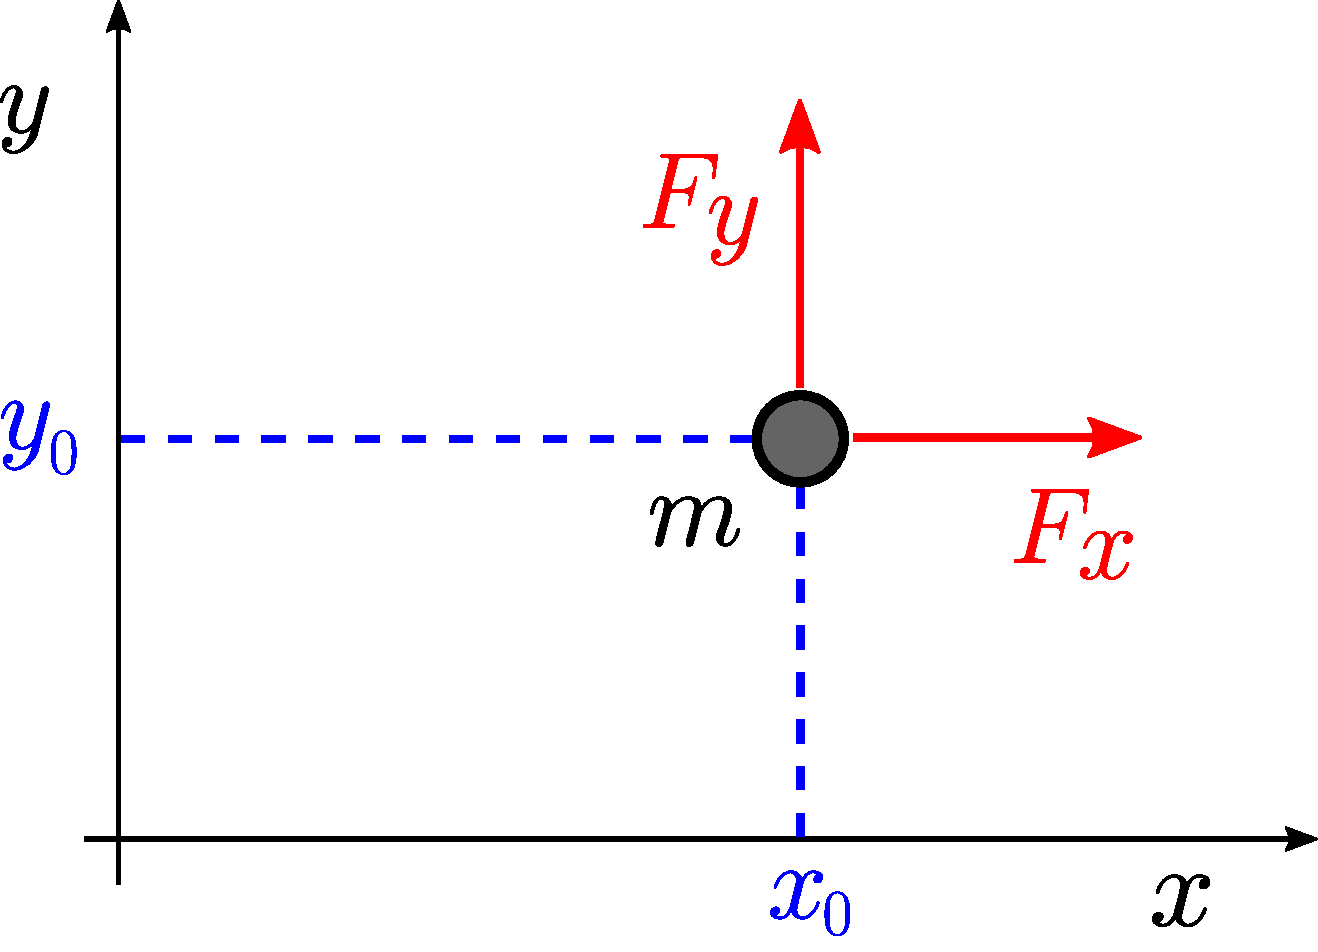
\includegraphics[width=0.4\textwidth]{figures/elements/mass-element}
\caption{Point mass element}
\label{fig:elements:point-mass}
\end{figure}

The equation of motion for this system can be written down directly by using Newton's second law of motion:
%
\begin{align}
m\cdot\ddot{x}_{0} &= F_x \\
m\cdot\ddot{y}_{0} &= F_y
\end{align}

Rearranging this into a matrix equation, using the nodal coordinates $\boldsymbol{u}(t) = \begin{bmatrix}x_0 & y_0\end{bmatrix}^\intercal$, results in

\begin{equation}
\underbrace{
\begin{bmatrix}
m & 0\\
0 & m
\end{bmatrix}
}_{\boldsymbol{M}}
\underbrace{
\begin{bmatrix}
\ddot{x}_0\\
\ddot{y}_0
\end{bmatrix}
}_{\boldsymbol{\ddot{u}}}
+
\underbrace{
\begin{bmatrix}
0\\
0
\end{bmatrix}
}_{\boldsymbol{Q}(\boldsymbol{u},\,\dot{\boldsymbol{u}})}
=
\underbrace{
\begin{bmatrix}
F_x\\
F_y
\end{bmatrix}
}_{\boldsymbol{P}(t)}.
\end{equation}

In this form we can immediately identify the element's mass matrix, internal forces (which are zero) and external forces.
Note that the mass matrix is diagonal, because there is no coupling between the two directions of motion.
Because the internal forces are zero, the tangent stiffness and damping matrices are zero as well:

\begin{equation}
\boldsymbol{K} = \frac{\partial \boldsymbol{Q}}{\partial \boldsymbol{u}} =
\begin{bmatrix}
0 & 0\\
0 & 0
\end{bmatrix},
\quad
\boldsymbol{D} = \frac{\partial \boldsymbol{Q}}{\partial \dot{\boldsymbol{u}}} =
\begin{bmatrix}
0 & 0\\
0 & 0
\end{bmatrix}
\end{equation}

\newpage
\section{Beam Element}

The beam elements are the core of the bow simulation, since they are used for modeling the static deflection and dynamic motion of the limbs.
There are various approaches to constructing geometrically nonlinear beam elements that can handle arbitrarily large displacements and rotations.
One such approach is the \textit{corotational formulation}, which is also what VirtualBow uses.
As a visual motivation for this method, consider the bow limb shown in figure~\ref{fig:beam-element-corotational-motivation-1}.
In this figure, a short segment of the limb is tracked from the initial unbraced state of the bow to full draw.
All shapes shown were exported from actual simulation results and are to scale.

\begin{figure}[h]
\centering
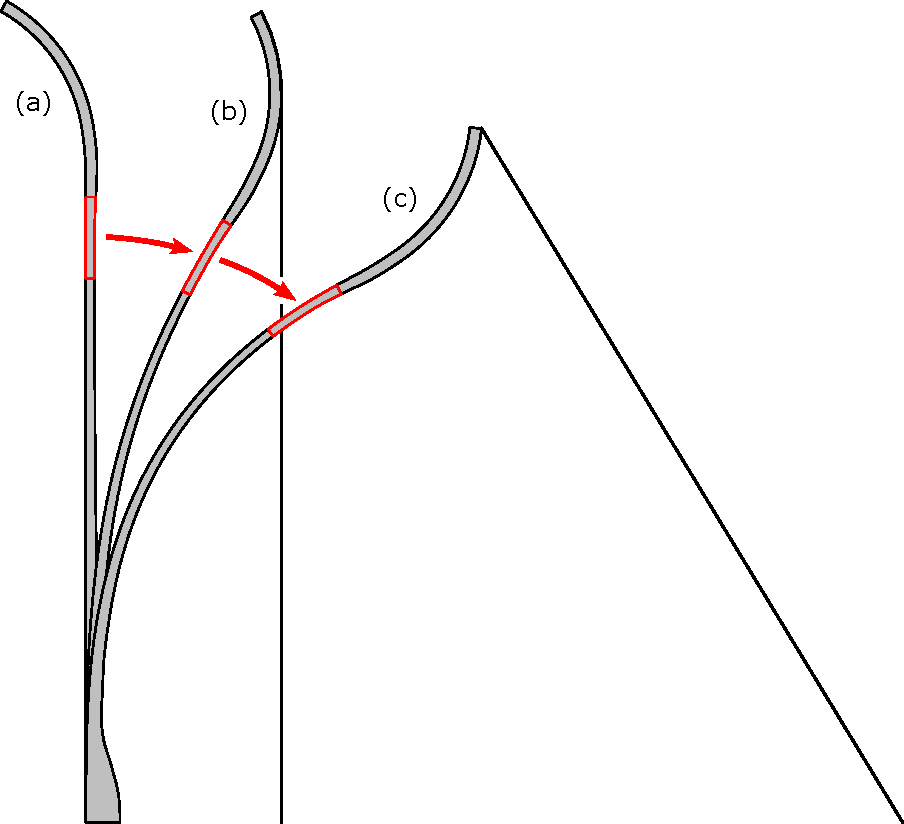
\includegraphics[width=0.8\textwidth]{figures/elements/beam-element-corotational-motivation-1}
\caption{Motion of a single limb segment from unbraced state~(a) over the braced state~(b) to full draw~(c)}
\label{fig:beam-element-corotational-motivation-1}
\end{figure}

The first observation is that the overall deflection of the limb as well as the motion of the tracked segment are indeed fairly large.
So there really is no hope for geometrically linear methods that treat the overall deflection as small.
Another observation though is that the tracked segment, while translating and rotating quite a bit, doesn't actually bend very much.
To confirm this, figure~\ref{fig:beam-element-corotational-motivation-2} shows the three segment shapes inside a common reference frame where the $\overline{x}$-axis passes through the center of the first and the last cross-section.

\begin{figure}[h]
\centering
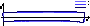
\includegraphics[width=1.0\textwidth]{figures/elements/beam-element-corotational-motivation-2}
\caption{Limb segment in the states (a), (b) and (c) within a common reference frame}
\label{fig:beam-element-corotational-motivation-2}
\end{figure}

And indeed, when viewed within this reference frame, the segment bends only very slightly.
It is easy to imagine that this elastic deformation would decrease even further if the length of the tracked segment was made shorter.
The large overall deflection of the limb seems to be the result of the compounding effect of all the small, local deformations.
The corotational formulation of beam elements makes use of this basic principle.
Within this formulation, each beam element is given a local frame of reference, similar to that shown in  figure~\ref{fig:beam-element-corotational-motivation-2}, that translates and rotates along with the element as it moves.
The actual motion of the element is then interpreted as the superposition of two parts:

\begin{enumerate}
\item A large, geometrically nonlinear, \textbf{rigid-body motion} of the element, as defined by the translation and rotation of its local reference frame.
\item A small, geometrically linear, \textbf{elastic deformation} of the element relative to its local reference frame.
\end{enumerate}

The big advantage of this approach is that the local, elastic deformations can be treated as linear, which is both conceptually more simple and computationally effective.
The resulting elements are valid for geometrically nonlinear problems where the overall deflection and rotation of a beam can be large as long as the local deformation within each element stays small.
We have already seen that this is a reasonable assumption for bows, and that it can always be made true by making the elements shorter and using more of them.

\newpage
\subsection{Corotational Formulation}

Let's now get a bit more precise and formulate this idea of a corotational reference frame in mathematical terms.
First we are going to look at a beam segment within its local frame of reference according to figure \ref{fig:beam-element-local-frame}.
The element is given two nodes, one at the left and one at the right.
The reference frame~$\{\overline{x},\,\overline{y}\}$ is positioned with its origin at the first node and oriented so that the~$\overline{x}$-axis passes through the second node.
This is not the only way that a corotational reference frame can be defined, but it seems to be the most common one~\cite{bib:le2011}\cite{bib:yaw2009} and has been compared favourably to other alternatives~\cite{bib:berzeri2001}.

\begin{figure}[h]
\centering
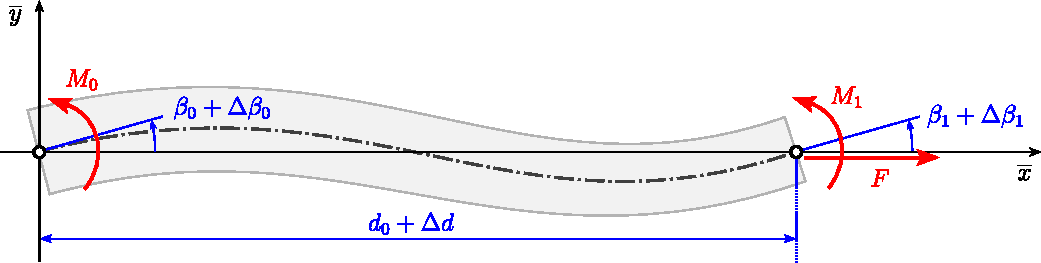
\includegraphics[width=1.0\textwidth]{figures/elements/beam-element-local-frame}
\caption{Element in its local reference frame}
\label{fig:beam-element-local-frame}
\end{figure}

The element is not assumed to be initially straight, or to have a constant cross-section for that matter.
Due to the possible initial curvature, its centerline has an initial angle of~$\beta_0$ at the first node and~$\beta_1$ at the second node, both measured against the $\overline{x}$-axis.
The initial distance between the two nodes is denoted by~$d_0$.

There are three degrees of freedom in which the nodes can move relative to the reference frame, complemented by three external forces:

\begin{enumerate}
\item Rotation of the first node, described by the angular change~$\Delta \beta_0$ and corresponding to the external moment $M_0$.
\item Rotation of the second node, described by the angular change~$\Delta \beta_1$ and corresponding to the external moment $M_1$.
\item Translation of the second node, described by the change in distance~$\Delta d$ and corresponding to the external force $F$.
\end{enumerate}

We combine the local elastic displacements into the vector~$\overline{\boldsymbol{u}} = \begin{bmatrix}\Delta d, & \Delta \beta_0, & \Delta \beta_1\end{bmatrix}^\intercal$ and the corresponding external forces into the vector~$\overline{\boldsymbol{P}} = \begin{bmatrix}F, & M_0, & M_1\end{bmatrix}^\intercal$.
According to the premise of the corotational formulation, the relationship between those forces and displacements within the local reference frame is linear.
We express this relationship as
%
\begin{equation}
\overline{\boldsymbol{P}} = \overline{\boldsymbol{Q}}(\boldsymbol{u}_{e},\,\dot{\boldsymbol{u}}_{e}) = \overline{\boldsymbol{K}}\overline{\boldsymbol{u}} + \overline{\boldsymbol{D}}\dot{\overline{\boldsymbol{u}}}, \label{eq:corotational-linear-forces}
\end{equation}

with the local internal forces $\overline{\boldsymbol{Q}}$, defined by the stiffness matrix~$\overline{\boldsymbol{K}} \in \mathbb{R}^{3\times 3}$ and the damping matrix~$\overline{\boldsymbol{D}} \in \mathbb{R}^{3\times 3}$, both of which are constant.
The derivation of those matrices from the beam's geometry and material properties will be shown later, for now we just take them as given.
Instead we will continue with developing the kinematic relations required for a corotational formulation.
Consider now the element in a state as shown in figure \ref{fig:beam-element-global-frame}, where its local reference frame has translated and rotated within the global reference frame.

\begin{figure}[h]
\centering
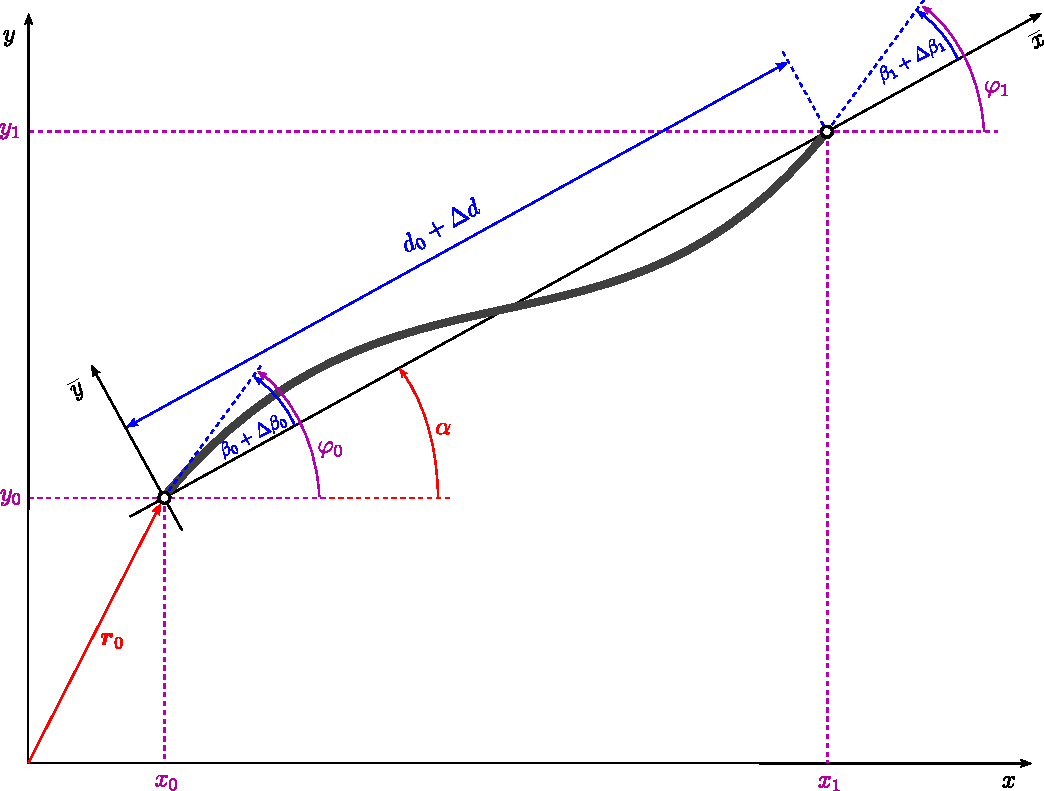
\includegraphics[width=1.0\textwidth]{figures/elements/beam-element-global-frame}
\caption{Element in the global reference frame}
\label{fig:beam-element-global-frame}
\end{figure}

Three different kinds of coordinates are shown in this figure:
The \textcolor{blue}{elastic displacements} of the element relative to its local reference frame that were defined earlier.
The \textcolor{red}{rigid-body motion} of the element's local reference frame, parameterized by the translation $\boldsymbol{r}_0$ of the reference frame's origin and its rotation angle $\alpha$.
And finally the \textcolor{magenta}{nodal positions and rotations} of the element in global coordinates.
These global positions and rotations are the coordinates in which we actually want to forumlate the equation of motion of the element:

\begin{equation}
\boldsymbol{u} = \begin{bmatrix}
x_{0}, & y_{0}, & \varphi_{0} & x_{1}, & y_{1}, & \varphi_{1}
\end{bmatrix}^\intercal
\end{equation}

These nodal coordinates fully characterize the motion of the element, including its rigid-body motion and its elastic deformation.
This is consistent with counting the degrees of freedom: three elastic displacement coordinates together with three rigid‑body coordinates yield six degrees of freedom, matching the number of nodal coordinates.
This means that, given the nodal coordinates, we can calculate the elastic and rigid-body coordinates.

The rigid-body translation $\boldsymbol{r}_0$ is given by the coordinates $x_0$ and $y_0$ of the first node.
The rigid-body rotation $\alpha$ can be calculated via $\arctan2$ as the angle of the $x'$-axis passing through the two nodes.
Let's first define some common terms, namely the differences~$\Delta x$ and~$\Delta y$ between the two nodes in $x$- and $y$-direction and their current distance~$d$: 

\begin{equation}
\begin{aligned}[c]
\Delta x &= x_1 - x_0, \\
\Delta y& = y_1 - y_0,
\end{aligned}
\qquad
\begin{aligned}[c]
d &= \sqrt{\Delta x^2 + \Delta y^2} \\ \\
\end{aligned}.
\end{equation}

The rigid-body coordinates are then expressed as

\begin{equation}
\boldsymbol{r}_{0} = \begin{bmatrix}
x_0 \\
y_0
\end{bmatrix},
\quad
\alpha = \arctan2\left(\frac{\Delta y}{\Delta x}\right).
\end{equation}

The elastic elongation~$\Delta d$ is the difference between the actual distance~$d$ of the nodes and the initial distance~$d_0$.
The elastic angular displacements~$\Delta \beta_0$ and~$\Delta \beta_1$ follow from considering the sum of angles at each node.
The relation between the elastic displacements~$\overline{\boldsymbol{u}}$ and the overall coordinates~$\boldsymbol{u}$ therefore turns out to be

\begin{equation}
\overline{\boldsymbol{u}}(\boldsymbol{u}) = \begin{bmatrix}
\Delta d \\ \Delta \beta_0 \\ \Delta \beta_1
\end{bmatrix}
=
\begin{bmatrix}
d - d_0 \\
\rm{normalize}\left(\varphi_0 - \beta_0 - \alpha\right) \\
\rm{normalize}\left(\varphi_1 - \beta_1 - \alpha\right)
\end{bmatrix}.
\end{equation}

One critical subtlety is required here: the resulting angular displacements need to be \textit{normalized}, i.e. wrapped to an interval of~$]-\pi,\,\pi]$.
That's because the nodal angles~$\varphi_0$,~$\varphi_1$ may be arbitrarily large, while the angle~$\alpha$ is clamped to an interval of~$]-\pi,\,\pi]$ due to the return value of the~$\arctan2$ function.
So the difference of those angles might be off by a multiple of $2\pi$, which is removed by the normalization.
The velocities of the elastic displacements are obtained by differentiating with the chain rule,

\begin{equation}
\dot{\overline{\boldsymbol{u}}}(\boldsymbol{u}) = \frac{\partial \overline{\boldsymbol{u}}}{\partial \boldsymbol{u}}\frac{d\boldsymbol{u}}{dt} = \boldsymbol{J}(\boldsymbol{u})\,\dot{\boldsymbol{u}},
\end{equation}

with the Jacobian $\boldsymbol{J}(\boldsymbol{u}) \in \mathbb{R}^{3 \times 6}$ that depends on the nodal coordinates and can be worked out as

\begin{equation}
\renewcommand\arraystretch{1.5}
\boldsymbol{J}(\boldsymbol{u}) =
\frac{\partial}{\partial\boldsymbol{u}}
\begin{bmatrix}
\Delta d \\
\Delta \beta_0 \\
\Delta \beta_1 \\
\end{bmatrix}
=
\begin{bmatrix}
-\frac{\Delta x}{d} & -\frac{\Delta y}{d} & 0 & \frac{\Delta x}{d} & \frac{\Delta y}{d} & 0 \\
-\frac{\Delta y}{d^2} & \frac{\Delta x}{d^2} & 1, & \frac{\Delta y}{d^2} & -\frac{\Delta x}{d^2} & 0 \\
-\frac{\Delta y}{d^2} & \frac{\Delta x}{d^2} & 0, & \frac{\Delta y}{d^2} & -\frac{\Delta x}{d^2} & 1 \\
\end{bmatrix}
\end{equation}

This kinematic relationship between nodal coordinates and elastic displacements is the key to formulating the element's internal forces in terms of its nodal coordinates.
Since the virtual work of the global internal forces $\boldsymbol{Q}$ must be equivalent to the virtual work of the local internal forces $\overline{\boldsymbol{Q}}$, we get the relation
%
\begin{align}
\delta\boldsymbol{u}^\intercal\boldsymbol{Q} &= \delta\overline{\boldsymbol{u}}^\intercal\overline{\boldsymbol{Q}} = \left(\boldsymbol{J}\,\delta\boldsymbol{u}\right)^\intercal\overline{\boldsymbol{Q}} = \delta\boldsymbol{u}^\intercal\boldsymbol{J}^\intercal\overline{\boldsymbol{Q}} \notag \\
\Rightarrow \boldsymbol{Q} &= \boldsymbol{J}^\intercal\overline{\boldsymbol{Q}} \label{eq:corotational-force-transform}
\end{align}

Stated in words: the transpose of the same Jacobian $\boldsymbol{J}$ that converts between local and global velocities also transforms between local and global forces.
By combining~\eqref{eq:corotational-force-transform} with the linear forces~\eqref{eq:corotational-linear-forces} and rewriting $\boldsymbol{u}_{e}$ and $\dot{\boldsymbol{u}}_{e}$ in terms of global coordinates, we get
the element's internal forces as
%
\begin{align}
\boldsymbol{Q}(\boldsymbol{u},\,\dot{\boldsymbol{u}}) &= \boldsymbol{J}^\intercal\overline{\boldsymbol{Q}} \notag \\
&= \boldsymbol{J}^\intercal\left(\overline{\boldsymbol{K}}\overline{\boldsymbol{u}} + \overline{\boldsymbol{D}}\dot{\overline{\boldsymbol{u}}}\right) \notag \\
&= \boldsymbol{J}^\intercal\overline{\boldsymbol{K}}\overline{\boldsymbol{u}}(\boldsymbol{u}) + \boldsymbol{J}^\intercal\overline{\boldsymbol{D}}\boldsymbol{J}\dot{\boldsymbol{u}}.
\end{align}

Note how the corotational formulation yields relatively simple, fully analytical expressions for the internal forces.
This stands in contrast to formulations in which the internal forces have to be evaluated numerically, often through Gaussian quadrature or related integration schemes.
The tangent stiffness and damping matrices are obtained by differentiation of the internal forces as

\begin{equation}
\boldsymbol{K} = \frac{\partial\boldsymbol{Q}}{\partial\boldsymbol{u}}, \qquad \boldsymbol{D} = \frac{\partial\boldsymbol{Q}}{\partial\dot{\boldsymbol{u}}}.
\end{equation}

Carrying out these derivatives is somewhat laborious but fairly straightforward, and it is therefore presented in full detail in Appendix~\ref{section:beam-element-stiffness-damping}.

Now only one final component of the element’s equation of motion is still missing: the inertia forces, i.e. the forces associated with the element's moving mass.
As already noted, the corotational formulation yields comparatively simple expressions for the internal forces.
The other side of that tradeoff, however, is that the inertia forces, when derived in a consistent way and without simplifications, become highly nonlinear and much more complex, see for example \cite{bib:le2011}.
They especially cannot be captured by a constant mass matrix, as has been the premise up to this point.
So instead of using a consistent mass matrix, we are going to construct a \textit{lumped mass matrix}, which is a common approximation where an element's mass and inertia is distributed, i.e. \textit{lumped}, to its nodes.
Suppose that, after this lumping process, each node carries a mass $m_i$ and a moment of inertia $J_i$, while the rest of the element is massless.
This leads to the following lumped mass matrix for our element:

\begin{equation}
\boldsymbol{M} = \begin{bmatrix}
m_0 & & & & \cdots & 0 \\
& m_0 & & & \iddots & \vdots\\
& & J_0 & & & \\
& & & m_1 & & \\
\vdots & \iddots & & & m_1 & \\
0 & \cdots & & & & J_1
\end{bmatrix},  \label{eq:corotational-mass-matrix}
\end{equation}

Like all lumped mass matrices, it is not only constant but also diagonal, which provides a very nice computational advantage.
If all element types used in a system have a diagonal mass matrix, then the overall system's mass matrix will be diagonal as well.
This greatly simplifies the computation of accelerations in dynamic analysis, for which the mass matrix has to be inverted.
Other than more general matrices, a diagonal matrix can be trivially inverted just by independently inverting its diagonal entries.
Of course, a lumped mass matrix remains an approximation and comes with certain drawbacks.
Its diagonal structure implies that any coupling between inertia forces in different directions is neglected.
Moreover, as we will see later, distributing a beam segment's mass and especially its rotational inertia to its nodes is not as straightforward as it may appear.
Several lumping strategies exist, each with its own limitations.
For VirtualBow, the tradeoffs that come with a lumped mass matrix make sense though.
While the dynamic bow simulation needs to be sufficiently accurate, its primary focus is the overall motion of the bow.
Capturing every higher harmonic of the limb's oscillation in detail is not essential for this purpose.
So a consistent, and therefore more accurate, mass matrix would likely offer little to no practical benefit while making the simulation more complicated than it needs to be.

With this we conclude the derivation of the corotational formulation for the beam element.
The next sections will fill in the missing details that have been handwaved here.
Specifically, the computation of the linear stiffness and damping matrices that were taken as given in~\eqref{eq:corotational-linear-forces} as well as the determination of the masses and inertias appearing in~\eqref{eq:corotational-mass-matrix}.

\newpage
\subsection{Castigliano's Second Theorem}

As a preparation for deriving the linear stiffness matrix of the beam element, we first revisit a very useful result from linear elasticity: \textit{Castigliano’s second theorem}.
This theorem provides a general method for computing the displacements of arbitrary linear‑elastic structures under external loads.
Wikipedia~\ref{bib:castigliano} states it as follows:

\textit{If the strain energy of a linearly elastic structure can be expressed as a function of generalised force $P_i$ then the partial derivative of the strain energy with respect to generalised force gives the generalised displacement $u_i$ in the direction of $P_i$.} (Notation adapted)

To illustrate this relationship between forces, displacements and potential energy, let's consider a bar under tension as shown in figure \ref{fig:castigliano-bar-1}.
It has an initial length of $l$ and a variable longitudinal stiffness $EA(s)$ that depends on the position $s \in [0,\,l]$ along the bar.
As a first exercise, let's compute the displacement~$u$ at the end of the bar that results from the force~$F$ being applied there.

\begin{figure}[h]
\centering
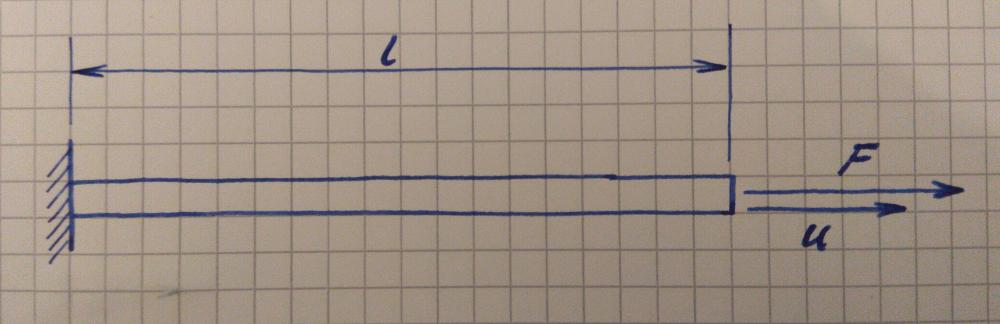
\includegraphics[width=0.6\textwidth]{figures/elements/castigliano-bar-1}
\caption{Bar with a tensile force applied at the free end}
\label{fig:castigliano-bar-1}
\end{figure}

First of all, the strain energy of a bar is given by

\begin{equation}
\Pi = \frac{1}{2}\int_{0}^{l}\frac{N^2}{EA}\,ds
\end{equation}

where $N(s)$ is the normal force at each cross-section along the length of the bar.
In this case it is easy to see that we have a constant normal force of $N(s) = F$.
According to Castigliano's theorem, the displacement $u$ in the direction of the force is

\begin{equation}
u = \frac{\partial \Pi}{\partial F} = \frac{\partial}{\partial F}\left(\frac{1}{2}\int_{0}^{l}\frac{F^2}{EA}\,ds\right) = \underbrace{\left(\int_{0}^{l}\frac{1}{EA}\,ds\right)}_{K^{-1}}F.
\end{equation}

By this we have identified the inverse $K^{-1}$ of the bar's stiffness in this loading case.
It is an integral over the initial length of the bar that takes the exact distribution of longitudinal stiffness into account.
If we assume $EA$ as constant for a quick sanity check, we get a stiffness of $K = EA/l$, which is the expected result for the stiffness of a uniform bar.
It is especially worth mentioning that we arrived at this result without any kinematic considerations, i.e. we didn't have to think about the distribution of strain in the bar due to the normal force and how that relates to the displacement $u$, which makes Castigliano's method very simple and elegant.
One apparent shortcoming is that this only gives us the displacement at the end of the bar, where the external force is applied, and nowhere else.
This limitation can be worked around by introducing additional "imaginary" forces at other points of interest and later setting them to zero after having worked out the associated displacements.

So as a second exercise, let's calculate the displacement $u^*$ at an arbitrary point $s^*$ within the bar as shown in figure \ref{fig:castigliano-bar-2} by introducing the imaginary auxiliary force $F^* = 0$.

\begin{figure}[h]
\centering
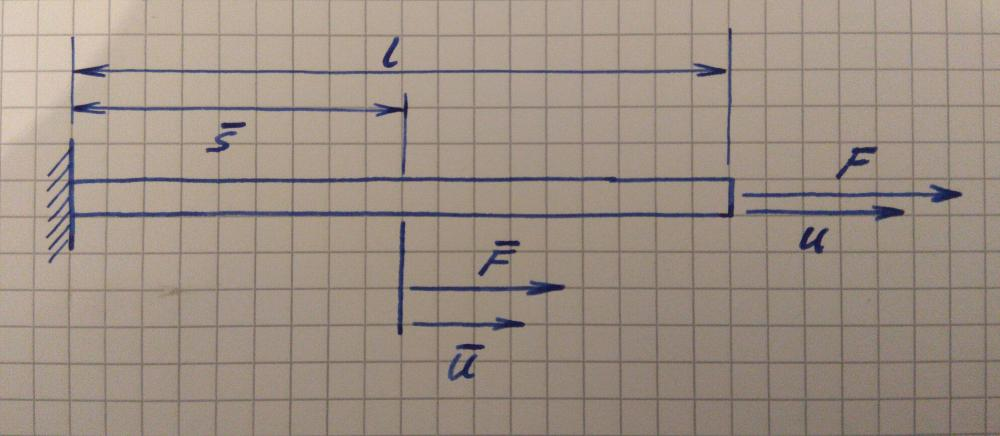
\includegraphics[width=0.6\textwidth]{figures/elements/castigliano-bar-2}
\caption{Bar with a tensile force and an auxiliary force}
\label{fig:castigliano-bar-2}
\end{figure}

The normal force over the length of the bar is now given by the piecewise function

\begin{equation}
N(s) = \begin{cases}
F + F^*, & \text{if}\ \ 0 \le s < s^* \\
F, & \text{if}\ \ s^* \le s \le l \\
\end{cases}
\end{equation}

Therefore the potential elastic energy becomes

\begin{equation}
\Pi = \frac{1}{2}\int_{0}^{l}\frac{N^2}{EA}\,ds = \frac{1}{2}\left(\int_{0}^{s^*}\frac{(F + F^*)^2}{EA}\,ds + \int_{s^*}^{l}\frac{F^2}{EA}\,ds\right)
\end{equation}

Application of Castigliano's theorem gives the displacement $u^*$ depending on the forces $F$ and $F^*$ as

\begin{equation}
u^* = \frac{\partial \Pi}{\partial F^*} = \frac{\partial}{\partial F^*}\left( \frac{1}{2} \int_{0}^{s^*}\frac{(F + F^*)^2}{EA}\,ds \right) = \left(\int_{0}^{s^*}\frac{1}{EA}\,ds \right)\left(F + F^*\right)
\end{equation}

The actual displacement is then obtained by setting the auxiliary force $F^*$ to zero, resulting in the actual displacement distribution within the bar,

\begin{equation}
u^*(s^*) = \left(\int_{0}^{s^*}\frac{1}{EA}\,ds \right)F.
\end{equation}

As a quick check, setting $s^* = l$ gives the same result for the end displacement as before.
Since Castigliano's method not only works for bars, but any linear-elastic structure, it will be an important tool for deriving the stiffness matrices required for the corotational formulation.

\subsection{Stiffness Matrix of a Beam Segment}

We can now use Castigliano's theorem for calculating the stiffness matrix and the deformation of a general, linear-elastic beam segment.
The segment can be initially curved and have variable cross-section properties along its length.
The only assumption we will make is that all displacements are small, so that we can apply linear-elastic theory to the problem.
Our approach will be similar to the one presented in~\cite{bib:marotta2018}.

\begin{figure}[h]
\centering
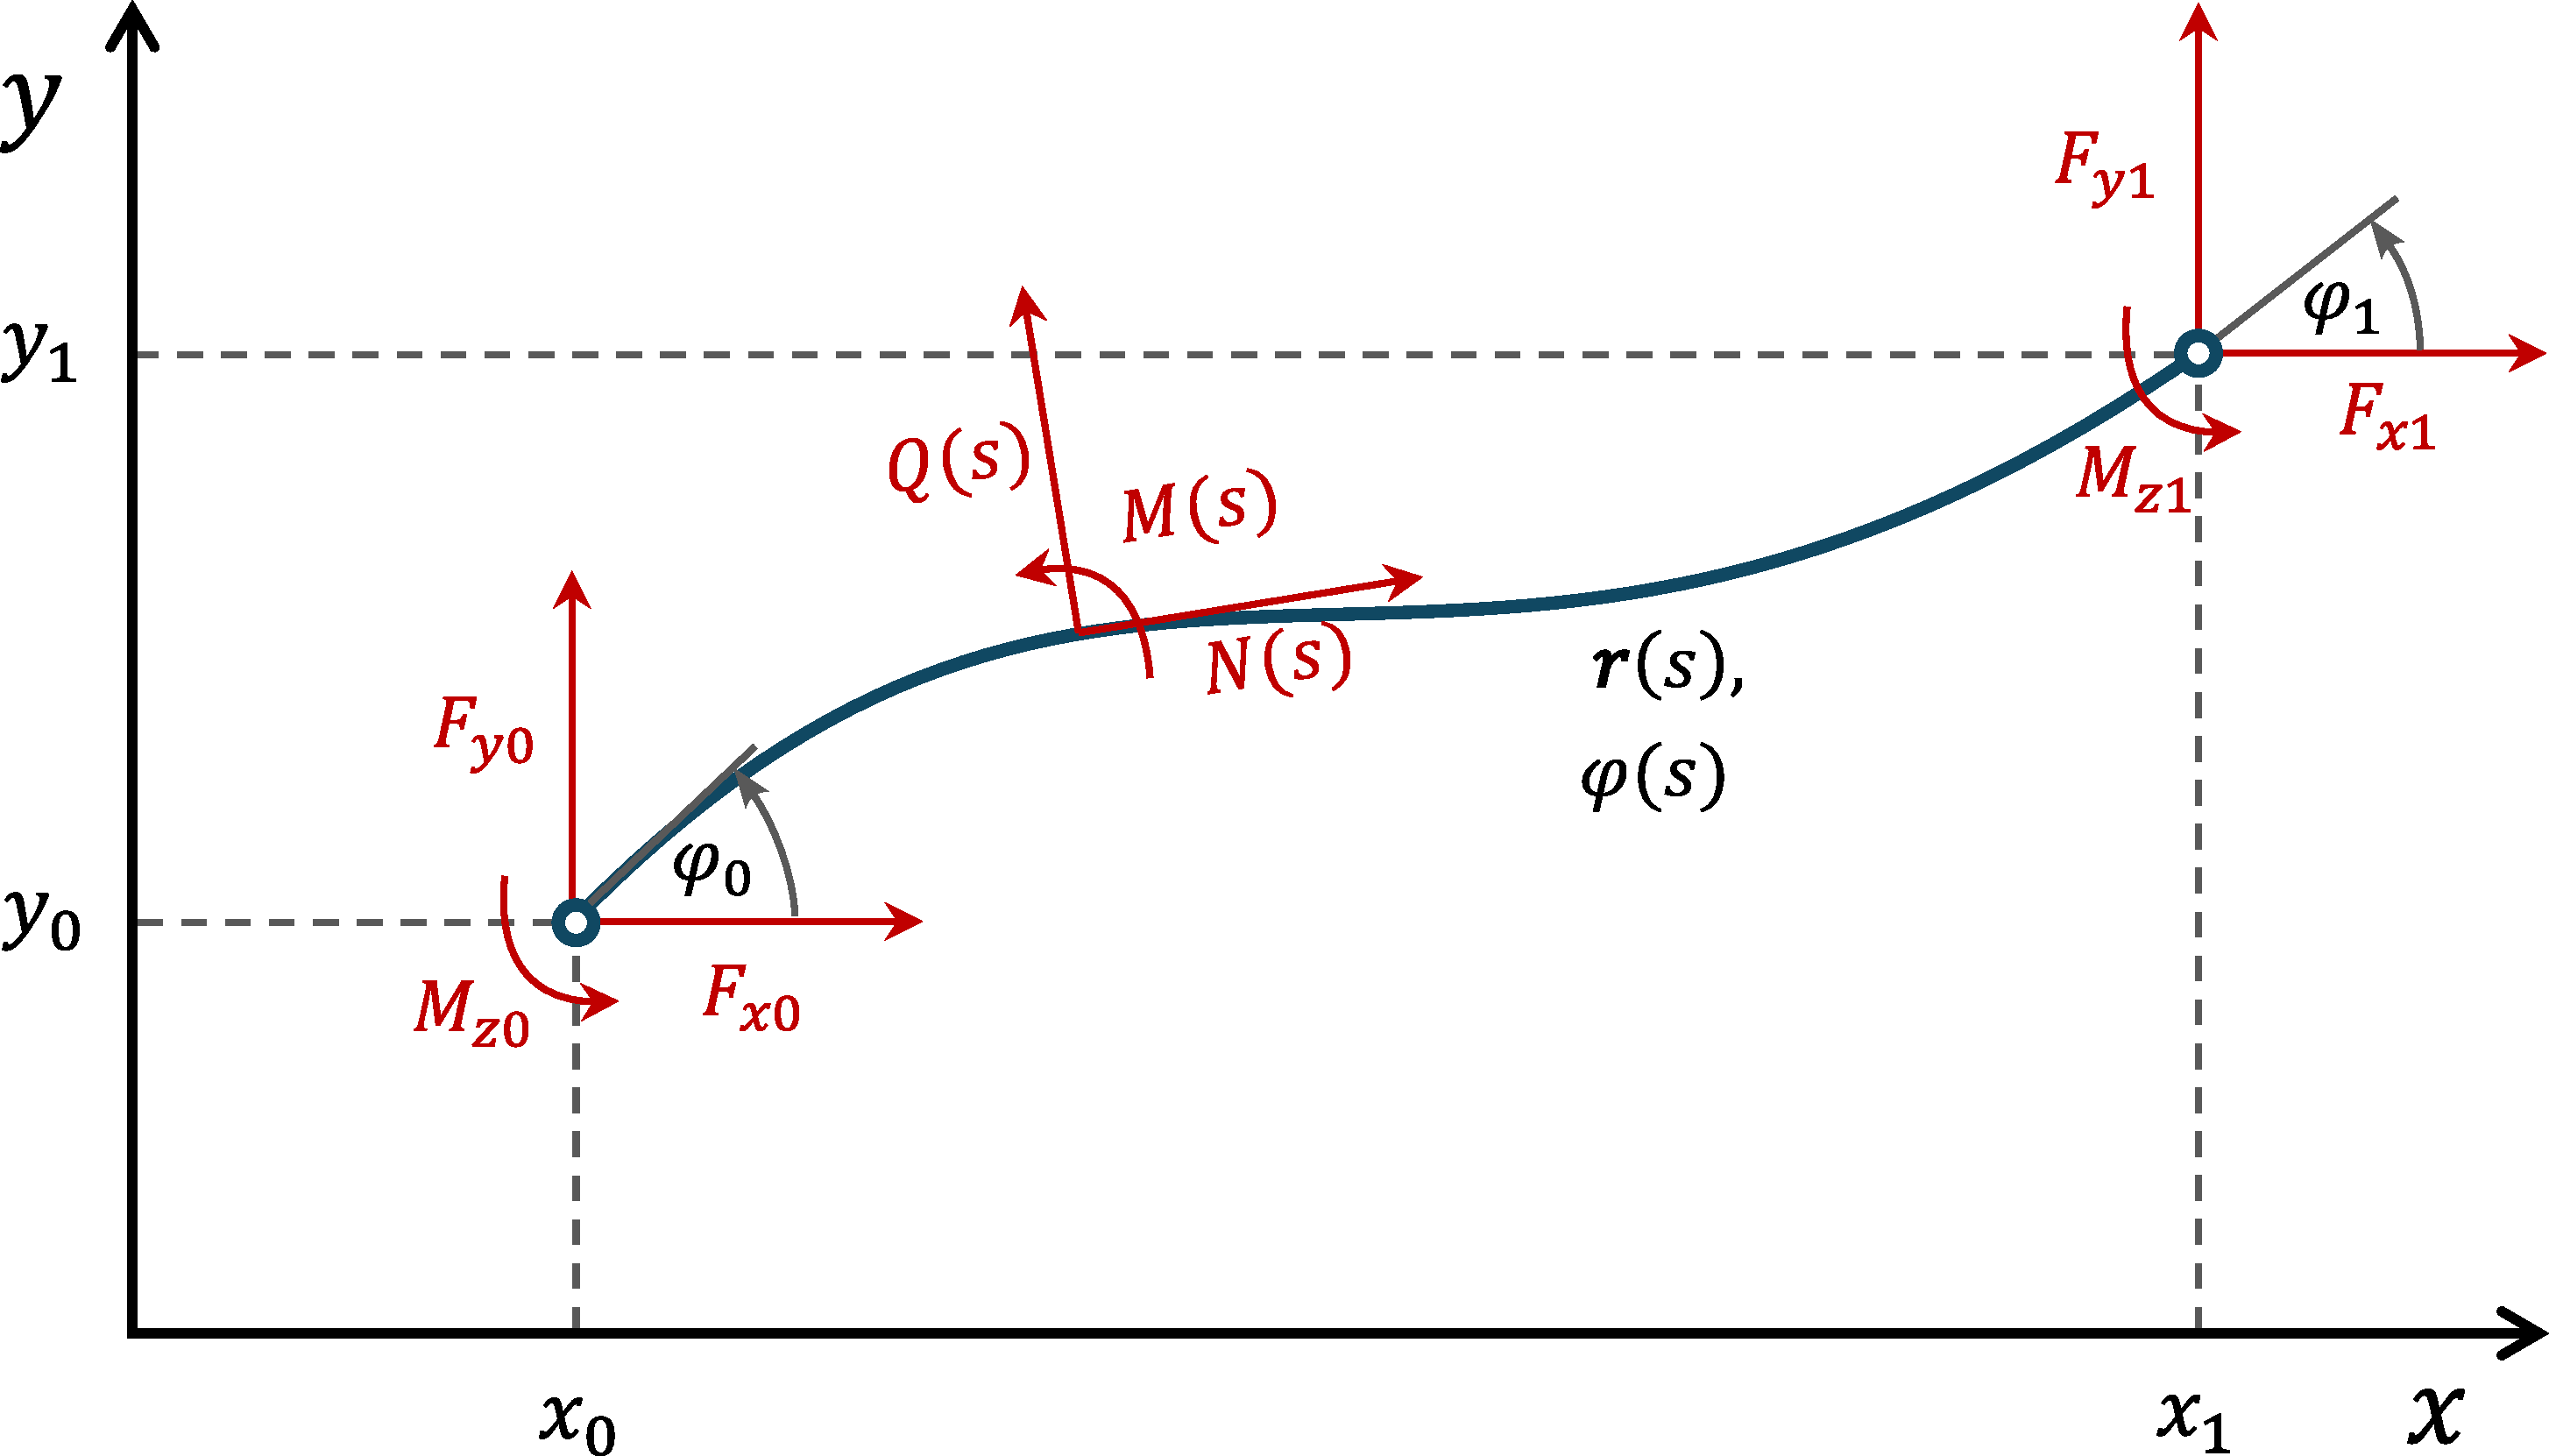
\includegraphics[width=0.8\textwidth]{figures/elements/beam-segment-linear}
\caption{Arbitrary beam segment with two nodes}
\label{fig:beam-segment-linear}
\end{figure}

Consider a beam segment as shown in figure $\ref{fig:beam-segment-linear}$.
It has two nodes and six nodal degrees of freedom, for which we will derive the complete $6 \times 6$ stiffness matrix.
The reduction to the $3 \times 3$ matrix required by our corotational formulation will be done later.
Its undeformed shape is described by the reference curve $\boldsymbol{r}(s) = \left[x(s),\,y(s)\right]^\intercal$ and the associated orientation angle $\varphi(s)$, where the parameter $s \in [s_0,\,s_1]$ is the arc length along the curve.
We combine the reference position and angle into a single function~$\boldsymbol{p}(s)$ and call the associated small displacements~$\Delta\boldsymbol{p}(s)$,

\begin{equation}
\boldsymbol{p}(s) = \begin{bmatrix}
x(s) \\
y(s) \\
\varphi(s)
\end{bmatrix},
\quad
\Delta\boldsymbol{p}(s) = \begin{bmatrix}
\Delta x(s) \\
\Delta y(s) \\
\Delta \varphi(s)
\end{bmatrix}.
\end{equation}

The stiffness properties of the cross-sections are given by their stiffness matrices $\boldsymbol{C}(s) \in \mathbb{R}^{3 \times 3}$ that are assumed to be known and establish a linear constitutive relation of the form

\begin{equation}
\underbrace{
\begin{bmatrix}
N \\
Q \\
M \\
\end{bmatrix}
}_{\boldsymbol{f}(s)}
=
\underbrace{
\begin{bmatrix}
C_{\varepsilon\varepsilon} & C_{\varepsilon\gamma} & C_{\varepsilon\kappa} \\
C_{\varepsilon\gamma} & C_{\gamma\gamma} & C_{\gamma\kappa} \\
C_{\varepsilon\kappa} & C_{\gamma\kappa} & C_{\kappa\kappa} \\
\end{bmatrix}
}_{\boldsymbol{C}(s)}
\underbrace{
\begin{bmatrix}
\varepsilon \\
\gamma \\
\kappa \\
\end{bmatrix}
}_{\boldsymbol{e}(s)} \label{eq:section-stiffness-matrix}
\end{equation}

between the cross section forces~$\boldsymbol{f}$ and the generalized strains~$\boldsymbol{e}$ at each length $s$ in the element.
The cross section forces consist of the normal force~$N$, the shear force~$Q$ and the bending moment~$M$ as shown in figure~\ref{fig:beam-segment-linear} while the strains consist of the elongation~$\varepsilon$ of the beam axis, the shear angle~$\gamma$ between the cross section and the beam axis and the curvature~$\kappa$ of the beam axis.
You may notice that we have introduced a bit of shear deformation here, even though the bow model was said to be based on Euler–Bernoulli theory earlier.
This is simply to keep the formulation more general and to prepare for future improvements.
Right now, VirtualBow does very little with this additional deformation.

The potential elastic energy (strain energy) of the beam segment, which we are going to need later, can be evaluated by integrating the product $\boldsymbol{f}^\intercal\boldsymbol{e}$ of section forces and strains over the beam's length and using the stiffness relation (\ref{eq:section-stiffness-matrix}) to eliminate the unknown strains:

\begin{equation}
\Pi = \frac{1}{2}\int_{s_0}^{s_1} \boldsymbol{f}^\intercal\boldsymbol{e}\,ds = \frac{1}{2}\int_{s_0}^{s_1} \boldsymbol{f}^\intercal\boldsymbol{C}^{-1}\boldsymbol{f}\,ds. \label{eq:section-potential-energy}
\end{equation}

We assign two nodes to this segment, one on the starting point~$s = s_0$ and one on the endpoint~$s = s_1$ of the curve.
Each node is given two translational degrees of freedom in $x$- and $y$-direction and an angular degree of freedom around the $z$-axis.
At each node, the respective forces and moments

\begin{equation}
\boldsymbol{F}_{0} = \begin{bmatrix}
F_{x,0} \\ F_{y,0} \\ M_{z,0}
\end{bmatrix},
\quad
\boldsymbol{F}_{1} = \begin{bmatrix}
F_{x,1} \\ F_{y,1} \\ M_{z,1}
\end{bmatrix}
\end{equation}

are applied, to which the beam segment reacts with the (small) nodal displacements

\begin{equation}
\Delta\boldsymbol{p}_{0} = \begin{bmatrix}
\Delta x_0 \\ \Delta y_0 \\ \Delta \varphi_0
\end{bmatrix},
\quad
\Delta\boldsymbol{p}_{1} = \begin{bmatrix}
\Delta x_1 \\ \Delta y_1 \\ \Delta \varphi_1
\end{bmatrix}
\end{equation}

in the respective directions of the forces/moments and relative to the initial state.
The goal is now to find the stiffness matrix of the segment, which describes the linear relationship between those forces and displacements.
The stiffness relation of the beam segment with respect to the combined nodal forces and displacements can be formally written as

\begin{equation}
\underbrace{
\begin{bmatrix}
\boldsymbol{F}_0 \\
\boldsymbol{F}_1 \\
\end{bmatrix}
}_{\boldsymbol{F}}
=
\underbrace{
\begin{bmatrix}
\boldsymbol{K}_{0,0} & \boldsymbol{K}_{0,1} \\
\boldsymbol{K}_{1,0} & \boldsymbol{K}_{1,1} \\
\end{bmatrix}
}_{\boldsymbol{K}}
\underbrace{
\begin{bmatrix}
\Delta\boldsymbol{p}_0 \\
\Delta\boldsymbol{p}_1 \\
\end{bmatrix}
}_{\boldsymbol{u}}
\end{equation}

with the overall stiffness matrix $\boldsymbol{K} \in \mathbb{R}^{6 \times 6}$ and four submatrices $\boldsymbol{K}_{ij} \in \mathbb{R}^{3 \times 3}$.
The overall forces $\boldsymbol{F}$ and displacements $\boldsymbol{u}$ have been chosen as the combination of the forces and displacements at nodes 0 and 1.
We can get a physical interpretation of the submatrices $\boldsymbol{K}_{ij}$ by keeping one of the nodes, respectively, fixed as shown in figure~\ref{fig:beam-segment-linear-cases}.

\begin{figure}[h]
\centering
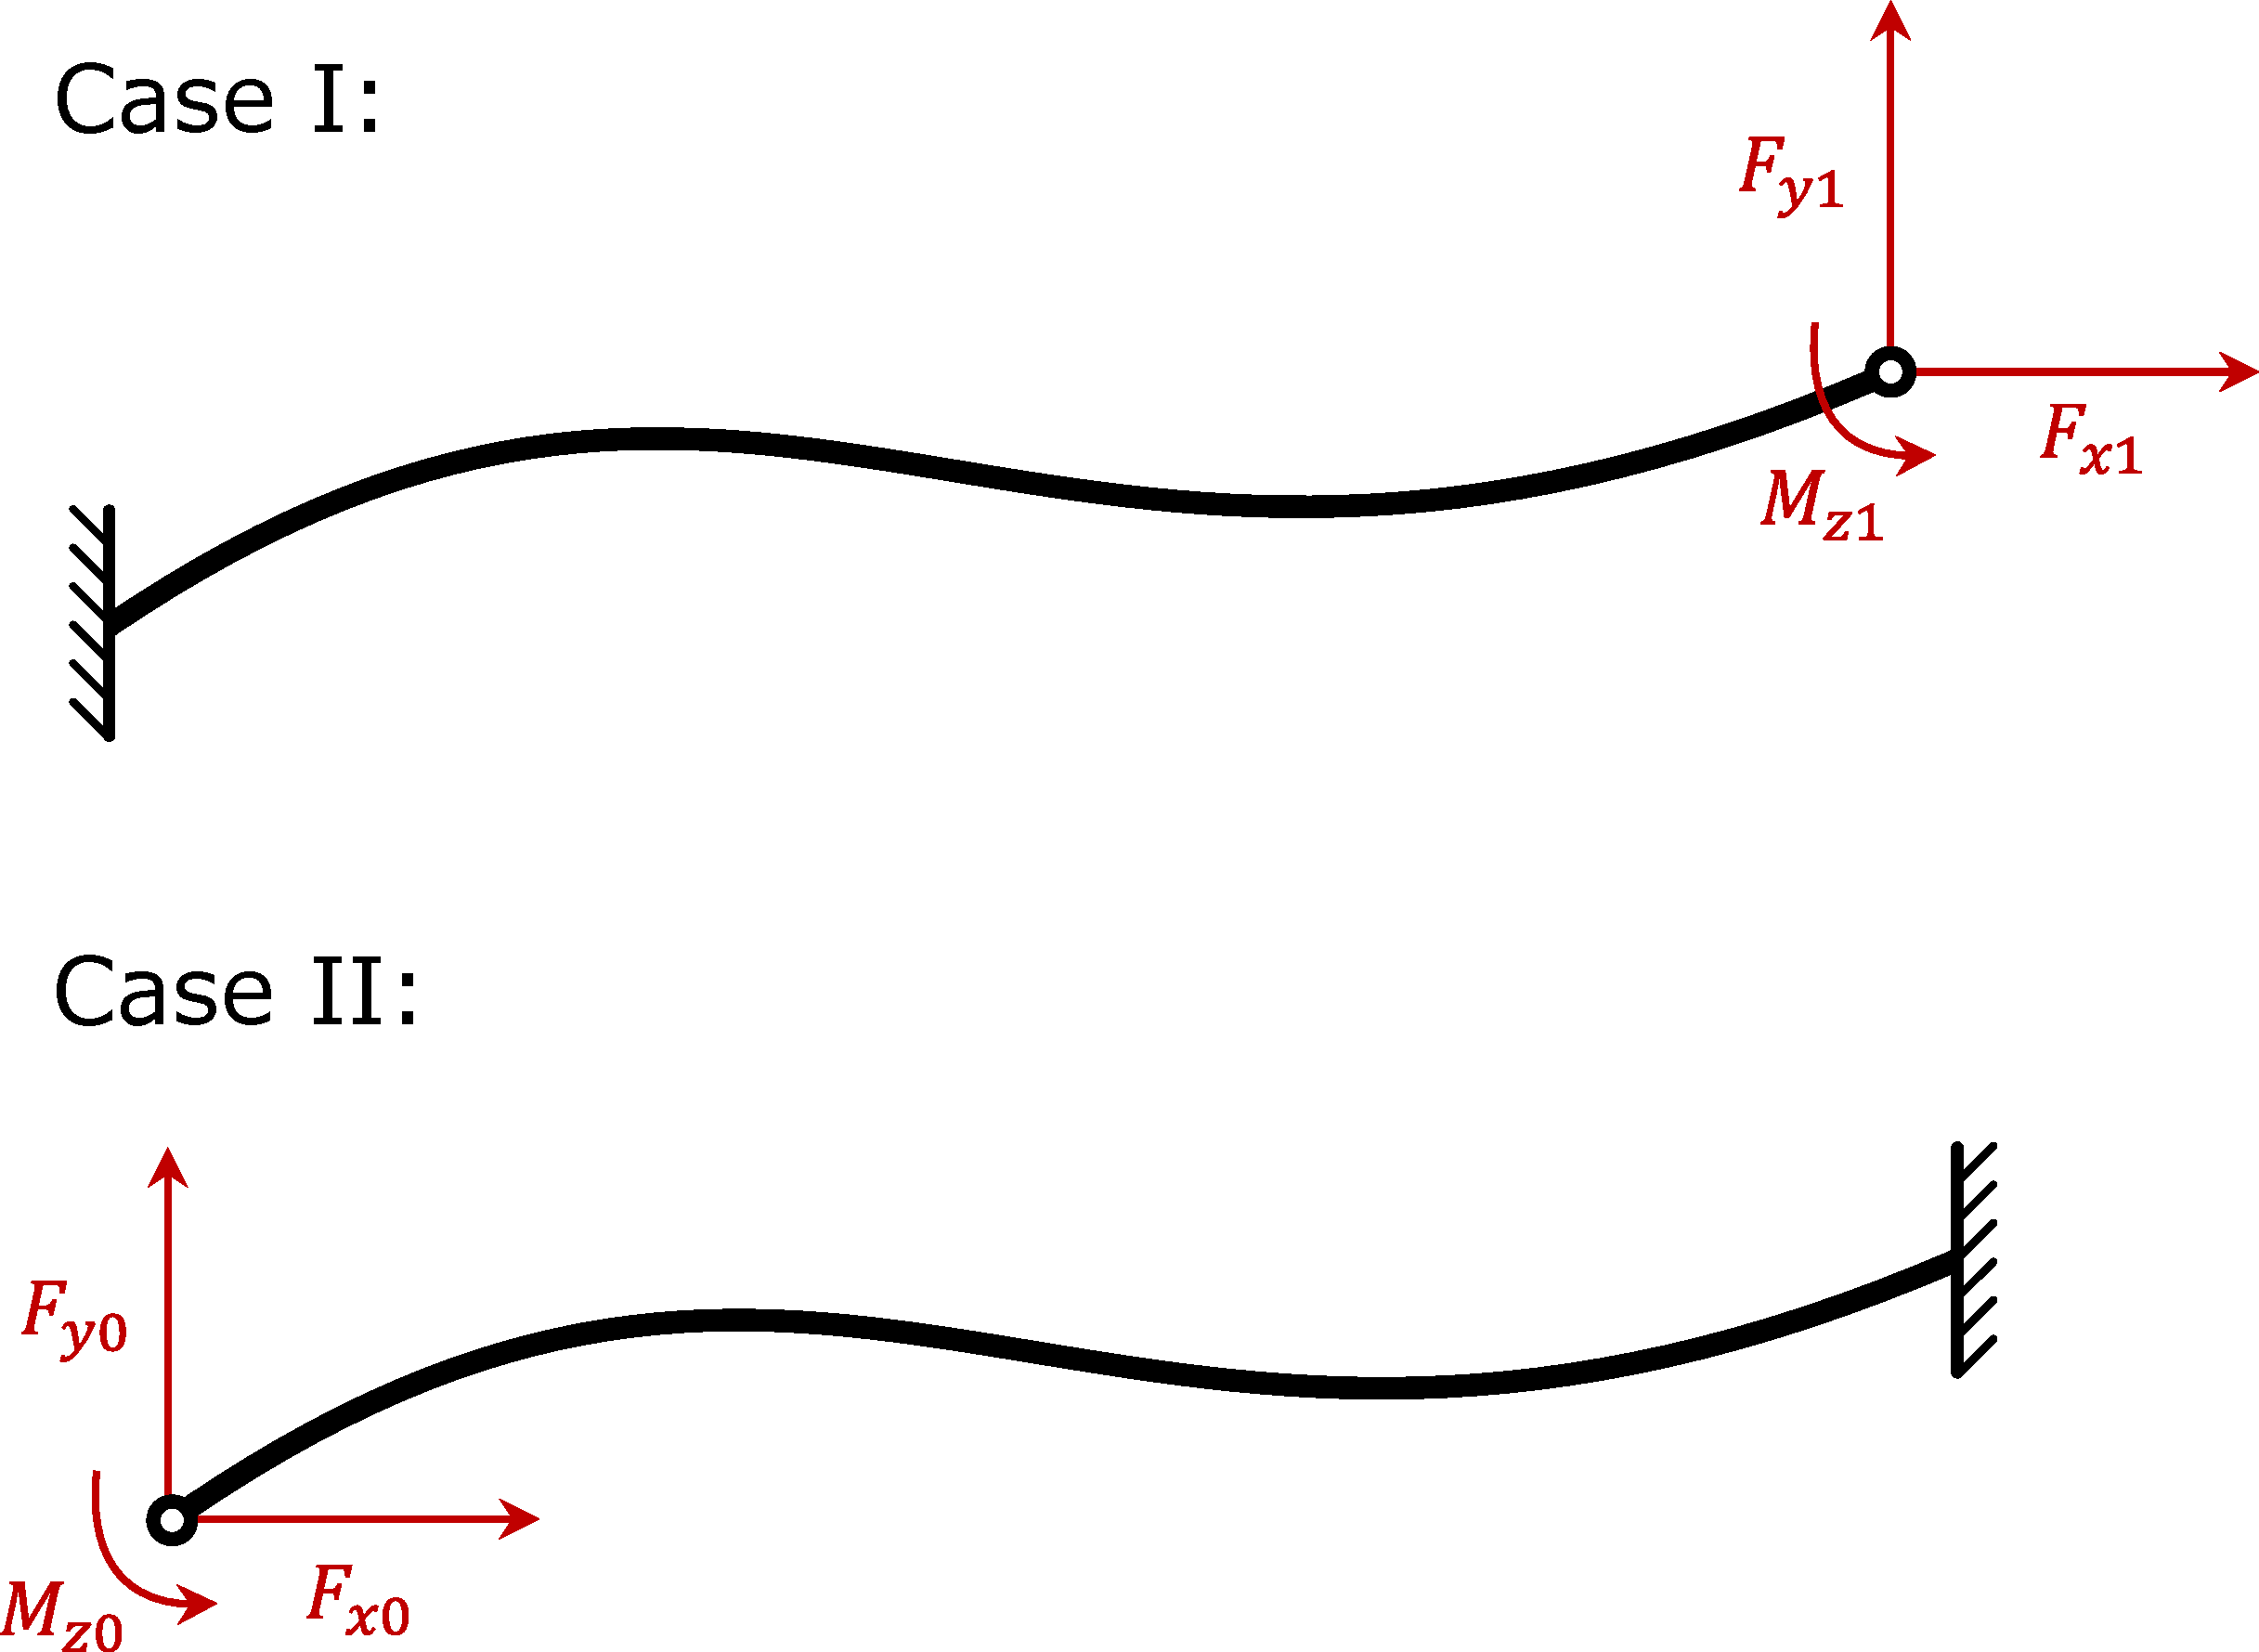
\includegraphics[width=0.6\textwidth]{figures/elements/beam-segment-linear-cases}
\caption{Beam segment with constrained nodes}
\label{fig:beam-segment-linear-cases}
\end{figure}

In \textbf{case I}, where the first node is being fixed ($\Delta\boldsymbol{p}_{0} = \boldsymbol{0}$), the resulting forces are
%
\begin{align}
\boldsymbol{F}_1 &= \boldsymbol{K}_{1,1}\,\Delta\boldsymbol{p}_1 \\
\boldsymbol{F}_0 &= \boldsymbol{K}_{0,1}\,\Delta\boldsymbol{p}_1
\end{align}

In \textbf{case II}, where the second node is being fixed, the resulting forces are
%
\begin{align}
\boldsymbol{F}_0 &= \boldsymbol{K}_{0,0}\,\Delta\boldsymbol{p}_0 \\
\boldsymbol{F}_1 &= \boldsymbol{K}_{1,0}\,\Delta\boldsymbol{p}_0
\end{align}

Put into words, the diagonal matrix blocks $\boldsymbol{K}_{0,0}$ and $\boldsymbol{K}_{1,1}$ relate the forces and displacements at the respective free node to each other, if the other node is restrained.
The off-diagonal blocks $\boldsymbol{K}_{1,0}$ and $\boldsymbol{K}_{0,1}$ relate the displacements at a free node to the forces at a restrained node.
This means that we can obtain the full stiffness matrix of the segment by analyzing those two simpler load cases and assembling the partial results in the end.

As a first step we note that the nodal forces $\boldsymbol{F}_0$ and $\boldsymbol{F}_1$ are not completely independent of each other, since they have to be in static equilibrium as a necessary condition for the element to be in equilibrium as a whole.
Balancing the forces and moments around node~1 gives us the three conditions
%
\begin{align}
x:\quad &F_{x,0} + F_{x,1} = 0 \\
y:\quad &F_{y,0} + F_{y,1} = 0 \\
z:\quad &M_{z,0} + M_{z,1} + F_{x,0}(y_1 - y_0) - F_{y,0}(x_1 - x_0) = 0
\end{align}

Solving for either $\boldsymbol{F}_0$ or $\boldsymbol{F}_1$ results in the following linear relationship between the nodal forces,

\begin{equation}
  \begin{split}
    \boldsymbol{F}_0 &= \boldsymbol{B}_{0,1}\cdot\boldsymbol{F}_1, \\
    \boldsymbol{F}_1 &= \boldsymbol{B}_{1,0}\cdot\boldsymbol{F}_0,
  \end{split}
\qquad
  \begin{split}
\boldsymbol{B}_{i,j} = \begin{bmatrix}
-1 & 0 & 0 \\
0 & -1 & 0 \\
y_j - y_i & x_i - x_j & -1
\end{bmatrix}.
  \end{split}
\end{equation}

with the static equilibrium matrix $\boldsymbol{B}_{i,j} = \boldsymbol{B}_{j,i}^{-1}$.
We can use this relationship to calculate the constraint forces at the clamped nodes in the cases I and II in order to obtain the off-diagonal stiffnesses $\boldsymbol{K}_{1,0}$ and $\boldsymbol{K}_{0,1}$ as follows,

\begin{align}
\boldsymbol{F}_0 &= \boldsymbol{B}_{0,1}\boldsymbol{F}_1 = \underbrace{\boldsymbol{B}_{0,1}\boldsymbol{K}_{1,1}}_{\boldsymbol{K}_{0,1}}\Delta\boldsymbol{p}_1, \\
\boldsymbol{F}_1 &= \boldsymbol{B}_{1,0}\boldsymbol{F}_0 = \underbrace{\boldsymbol{B}_{1,0}\boldsymbol{K}_{0,0}}_{\boldsymbol{K}_{1,0}}\Delta\boldsymbol{p}_0.
\end{align}

This means that we only have to determine the diagonal blocks $\boldsymbol{K}_{0,0}$ and $\boldsymbol{K}_{1,1}$ from load cases I and II and then use the results above in order to complete the stiffness matrix.

\subsubsection*{Stiffness and Displacements for Case I}

The beam is clamped at node 0 and a force is applied at node 1.
Due to static equilibrium, the distribution of cross section forces in the beam for an external force~$\boldsymbol{F}_\eta$ that is applied at the length~$s_\eta$ with~$\eta \in [0,\,1]$ are found to be

\begin{equation}
\underbrace{
\begin{bmatrix}
N \\ Q \\ M
\end{bmatrix}
}_{\boldsymbol{f}^{\mathrm{I}}_{\eta}(s)}
=
\underbrace{
\begin{bmatrix}
\cos(\varphi(s)) & \sin(\varphi(s)) & 0 \\
-\sin(\varphi(s)) & \cos(\varphi(s)) & 0 \\
y(s) - y(s_\eta) & x(s_\eta) - x(s) & 1
\end{bmatrix}
}_{\boldsymbol{H}_{\eta}(s)}
\underbrace{
\begin{bmatrix}
F_{x,\eta} \\ F_{y,\eta} \\ M_{z,\eta}
\end{bmatrix}
}_{\boldsymbol{F}_\eta} \label{eq:section-static-equilibrium}
\end{equation}

Combining the nodal force $\boldsymbol{F}_1$ at $s_1$ and the auxiliary force $\boldsymbol{F}_\eta$ at $s_\eta$ (used for Castigliano's theorem and later set to zero) we get the total cross section force

\begin{equation}
\boldsymbol{f}^{\mathrm{I}}(s) = \begin{cases}
\boldsymbol{H}_{1}(s)\boldsymbol{F}_1 + \boldsymbol{H}_{\eta}(s)\boldsymbol{F}_\eta, & \text{if}\ \ s_0 \le s < s_\eta \\
\boldsymbol{H}_{1}(s)\boldsymbol{F}_1, & \text{if}\ \ s_\eta \le s \le s_1 \\
\end{cases}
\end{equation}

The strain energy for this loadcase according to (\ref{eq:section-potential-energy}) is therefore

\begin{equation}
\Pi^{\mathrm{I}} = \frac{1}{2}\left(\int_{s_0}^{s_\eta} \left(\boldsymbol{H}_{1}\boldsymbol{F}_1 + \boldsymbol{H}_{\eta}\boldsymbol{F}_\eta\right)^\intercal\boldsymbol{C}^{-1}\left(\boldsymbol{H}_{1}\boldsymbol{F}_1 + \boldsymbol{H}_{\eta}\boldsymbol{F}_\eta\right)\,ds + \int_{s_\eta}^{s_1} \left(\boldsymbol{H}_{1}\boldsymbol{F}_1\right)^\intercal\boldsymbol{C}^{-1}\left(\boldsymbol{H}_{1}\boldsymbol{F}_1\right)\,ds\right)
\end{equation}

and the displacements $\Delta\boldsymbol{p}_\eta$ at position $s_\eta$ are obtained by Castigliano's theorem as

\begin{align}
\Delta\boldsymbol{p}^{\mathrm{I}}_\eta &= \frac{\partial \Pi^{\mathrm{I}}}{\partial \boldsymbol{F}_\eta}\Bigg|_{\boldsymbol{F}_\eta = 0} = \frac{\partial}{\partial \boldsymbol{F}_\eta}\left(\frac{1}{2}\int_{s_0}^{s_\eta} \left(\boldsymbol{H}_{1}\boldsymbol{F}_1 + \boldsymbol{H}_{\eta}\boldsymbol{F}_e\right)^\intercal\boldsymbol{C}^{-1}\left(\boldsymbol{H}_{1}\boldsymbol{F}_1 + \boldsymbol{H}_{\eta}\boldsymbol{F}_\eta\right)\,ds\right)\Bigg|_{\boldsymbol{F}_\eta = 0} \notag \\
&= \underbrace{\left(\int_{s_0}^{s_\eta} \boldsymbol{H}_\eta^\intercal\boldsymbol{C}^{-1}\boldsymbol{H}_1\,ds\right)}_{\boldsymbol{K}^{-1}_{1,\eta}}\boldsymbol{F}_1.
\end{align}

The inverse stiffness matrix $\boldsymbol{K}^{-1}_{1,1}$ for the right node follows for $\eta = 1$.

\subsubsection*{Stiffness and Displacements for Case II}

In the second case, where the beam is clamped at node 1 and the force is applied at node 0 instead, the section forces turn out to be

\begin{equation}
\underbrace{
\begin{bmatrix}
N \\ Q \\ M
\end{bmatrix}
}_{\boldsymbol{f}^{\mathrm{II}}_{\eta}(s)}
=
\underbrace{
\begin{bmatrix}
-\cos(\varphi(s)) & -\sin(\varphi(s)) & 0 \\
\sin(\varphi(s)) & -\cos(\varphi(s)) & 0 \\
y(s_\eta) - y(s) & x(s) - x(s_\eta) & -1
\end{bmatrix}
}_{-\boldsymbol{H}_{\eta}(s)}
\underbrace{
\begin{bmatrix}
F_{x,\eta} \\ F_{y,\eta} \\ M_{z,\eta}
\end{bmatrix}
}_{\boldsymbol{F}_\eta}, \label{eq:section-static-equilibrium}
\end{equation}

\begin{equation}
\boldsymbol{f}^{\mathrm{II}}(s) = \begin{cases}
-\boldsymbol{H}_{0}(s)\boldsymbol{F}_0, & \text{if}\ \ s_0 \le s \le s_\eta \\
-\boldsymbol{H}_{0}(s)\boldsymbol{F}_0 - \boldsymbol{H}_{\eta}(s)\boldsymbol{F}_\eta, & \text{if}\ \ s_\eta \le s < s_1 \\
\end{cases}.
\end{equation}

The strain energy follows as

\begin{equation}
\Pi^{\mathrm{II}} = \frac{1}{2}\left(\int_{s_0}^{s_\eta} \left(\boldsymbol{H}_{0}\boldsymbol{F}_0\right)^\intercal\boldsymbol{C}^{-1}\left(\boldsymbol{H}_{0}\boldsymbol{F}_0\right)\,ds + \int_{s_\eta}^{s_1} \left(\boldsymbol{H}_{0}\boldsymbol{F}_0 + \boldsymbol{H}_{\eta}\boldsymbol{F}_\eta\right)^\intercal\boldsymbol{C}^{-1}\left(\boldsymbol{H}_{0}\boldsymbol{F}_0 + \boldsymbol{H}_{\eta}\boldsymbol{F}_\eta\right)\,ds\right)
\end{equation}

and finally, the displacements according to Castigliano's theorem are

\begin{align}
\Delta\boldsymbol{p}^{\mathrm{II}}_\eta &= \frac{\partial \Pi^{\mathrm{II}}}{\partial \boldsymbol{F}_\eta}\Bigg|_{\boldsymbol{F}_\eta = 0} = \frac{\partial}{\partial \boldsymbol{F}_\eta}\left(\frac{1}{2}\int_{s_\eta}^{s_1} \left(\boldsymbol{H}_{0}\boldsymbol{F}_0 + \boldsymbol{H}_{\eta}\boldsymbol{F}_\eta\right)^\intercal\boldsymbol{C}^{-1}\left(\boldsymbol{H}_{0}\boldsymbol{F}_0 + \boldsymbol{H}_{\eta}\boldsymbol{F}_\eta\right)\,ds\right)\Bigg|_{\boldsymbol{F}_\eta = 0} \notag \\
&= \underbrace{\left(\int_{s_\eta}^{s_1} \boldsymbol{H}_\eta^\intercal\boldsymbol{C}^{-1}\boldsymbol{H}_0\,ds\right)}_{\boldsymbol{K}^{-1}_{0,\eta}}\boldsymbol{F}_0
\end{align}

and the stiffness matrix $\boldsymbol{K}^{-1}_{0,0}$ for the left node follows for $\eta = 0$.

\subsubsection*{Combined Stiffness and Displacements}

Combining all previous results, the four components of the full stiffness matrix are computed as
%
\begin{align}
\boldsymbol{K}^{-1}_{0,0} &= \int_{s_0}^{s_1} \boldsymbol{H}_0^\intercal\boldsymbol{C}^{-1}\boldsymbol{H}_0\,ds & \boldsymbol{K}^{-1}_{1,1} &= \int_{s_0}^{s_1} \boldsymbol{H}_1^\intercal\boldsymbol{C}^{-1}\boldsymbol{H}_1\,ds \\
\boldsymbol{K}_{1,0} &= \boldsymbol{B}_{1,0}\boldsymbol{K}_{0,0} & \boldsymbol{K}_{0,1} &= \boldsymbol{B}_{0,1}\boldsymbol{K}_{1,1}
\end{align}

Alternatively, since the stiffness matrtix must be symmetric, the relation $\boldsymbol{K}_{0,1} = \boldsymbol{K}_{1,0}^\intercal$ can be used for calculating one of the off-diagonal blocks in terms of the other.
Verifying that this is true is left as an exercise to the reader \texttt{;)}
The full displacements of the beam segment under forces at both nodes is obtained by adding the displacements from both constrained cases due to linear superposition,

\begin{equation}
\Delta\boldsymbol{p}_{\eta} = \boldsymbol{K}_{0,\eta}^{-1}\,\boldsymbol{F}_0 + \boldsymbol{K}_{1,\eta}^{-1}\,\boldsymbol{F}_1.
\end{equation}

Expressed in terms of the nodal displacements $\boldsymbol{u}$, this turns into
%
\begin{align}
\Delta\boldsymbol{p}_{\eta} &= \boldsymbol{K}_{0,\eta}^{-1}\boldsymbol{K}_{0,0}\boldsymbol{u}_0 + \boldsymbol{K}_{1,\eta}^{-1}\boldsymbol{K}_{1,1}\boldsymbol{u}_1 \notag \\
&=
\underbrace{
\left[\boldsymbol{K}_{0,\eta}^{-1}\boldsymbol{K}_{0,0} \ \vert\ \boldsymbol{K}_{1,\eta}^{-1}\boldsymbol{K}_{1,1}\right]
}_{\boldsymbol{E}_{u,\eta}}
\underbrace{
\begin{bmatrix}
\boldsymbol{u}_0 \\
\boldsymbol{u}_1
\end{bmatrix}
}_{\boldsymbol{u}} = \boldsymbol{E}_{u,\eta}\cdot\boldsymbol{u}\label{eq:beam-segment-displacement-eval}
\end{align}

with a displacement evaluation matrix $\boldsymbol{E}_{u,\eta}$.
We can simplify the computation of the matrices $\boldsymbol{K}_{0,\eta}^{-1}$ and $\boldsymbol{K}^{-1}_{1,\eta}$ by realizing that $\boldsymbol{H}_0$ and $\boldsymbol{H}_1$ are related by the static equilibrium matrix $\boldsymbol{B}_{i,j}$ as

\begin{equation}
\boldsymbol{H}_\eta(s) = -\boldsymbol{H}_0(s)\boldsymbol{B}_{\eta,0}
\end{equation}

Using this, the flexibility matrices can be written by using the same expression inside the integral, but integrated over different bounds:
%
\begin{align}
\boldsymbol{K}_{0,\eta}^{-1} &= -\boldsymbol{B}_{0,\eta}^\intercal\left(\int_{s_\eta}^{s_1} \boldsymbol{H}_0^\intercal\boldsymbol{C}^{-1}\boldsymbol{H}_0\,ds\right) \\
\boldsymbol{K}^{-1}_{1,\eta} &= \boldsymbol{B}_{0,\eta}^\intercal\left(\int_{s_0}^{s_\eta} \boldsymbol{H}_0^\intercal\boldsymbol{C}^{-1}\boldsymbol{H}_0\,ds\right)\boldsymbol{B}_{0,1}.
\end{align}

Note that until here those results are exact, in the sense that no further simplifications within the linear-elastic beam theory have been made.
The integrals over the segment's length account for arbitrary variations of shape and cross-section properties.
The integration itself is done numerically though in the actual implementation, because accounting for all kinds of shapes and cross-sections analytically would be too complicated.
The integration interval $[s_0,\,s_1]$ is divided into $n$ subintervals, and the integral for each subinterval is approximated using \textit{Simpson's rule}.
To obtain the resuired integrals from above, these partial results are added as needed.
Since the stiffness matrix and the evaluation matrices are constant, they have to be computed only once prior to the simulation.
Therefore the integrarion is not performance-critical and can be done fairly accurately with small numerical tolerances.

%\subsubsection*{Evaluation of section forces and strains}

%\textcolor{red}{TODO: Try to make these work or document actual evaluation}

%The stiffness matrix relates the nodal forces and displacements to each other, but it doesn't tell us anything about what happens within the beam segment in terms of forces and strains.
%For the section forces we can use equation (\ref{eq:section-static-equilibrium}) and the total stiffness equation (\ref{eq:segment-stiffness-matrix}) to get

%\begin{equation}
%\boldsymbol{f}(s) = \boldsymbol{H}(s)\boldsymbol{F}_{1} = \underbrace{\boldsymbol{H}(s)\left[\boldsymbol{K}_{10},\,\boldsymbol{K}_{11}\right]}_{\boldsymbol{E}_f(s)}\boldsymbol{u}.
%\end{equation}

%So the section forces at any length $s$ are linearly related to the nodal displacements~$\boldsymbol{u}$ via the matrix~$\boldsymbol{E}_f(s)$, which we will call the force evaluation matrix.
%Knowing the cross section forces, the strains can be computed from (\ref{eq:section-stiffness-matrix}) by inverting the section's stiffness matrix,

%\begin{equation}
%\boldsymbol{e}(s) = \boldsymbol{C}^{-1}(s)\boldsymbol{f}(s) = \underbrace{\boldsymbol{C}^{-1}(s)\boldsymbol{E}_f(s)}_{\boldsymbol{E}_e(s)}\boldsymbol{u}.
%\end{equation}

%In this case the relation to the displacements~$\boldsymbol{u}$ is given by the strain evaluation matrix~$\boldsymbol{E}_e(s)$.
%Both of these matrices can be pre-computed for certain points of interest within the beam segment.
%The actual evaluation of forces and strains is then only a matrix multiplication with the current nodal displacements.

\subsubsection*{Corotational Reference Frame}

We now have a general~$6 \times 6$ stiffness matrix of a beam segment in global coordinates, but according to figure~\ref{fig:beam-element-global-frame} we need the stiffness matrix relative to a coordinate system that is rotated by the initial angle of~$\alpha(t=0)$ and reduced to the three local coordinates~$\overline{\boldsymbol{u}} = \begin{bmatrix}\Delta d, & \Delta \beta_0, & \Delta \beta_1\end{bmatrix}^\intercal$.
The relation between the segment's full displacements~$\boldsymbol{u}$ and the local coordinates is found to be

\begin{equation}
\boldsymbol{u} =
\begin{bmatrix}
\Delta x_0 \\ \Delta y_0 \\ \Delta \varphi_0 \\ \Delta x_1 \\ \Delta y_1 \\ \Delta \varphi_1
\end{bmatrix}
=
\begin{bmatrix}
0 & 0 & 0 \\
0 & 0 & 0 \\
0 & 1 & 0 \\
\cos(\alpha) & 0 & 0 \\
\sin(\alpha) & 0 & 0 \\
0 & 0 & 1 \\
\end{bmatrix}
\begin{bmatrix}
\Delta d \\ \Delta \beta_0 \\ \Delta \beta_1
\end{bmatrix}
=
\boldsymbol{T}
\overline{\boldsymbol{u}}
\end{equation}

with the transformation matrix~$\boldsymbol{T}$.
The transformed stiffness matrix is then~$\overline{\boldsymbol{K}} = \boldsymbol{T}^\intercal\boldsymbol{K}\boldsymbol{T}$.
Similarly, the evaluation matrices in the corotated frame are~$\overline{\boldsymbol{E}} = \boldsymbol{E}\boldsymbol{T}$.

But we don't only want to transform things into the corotational frame, we also want to transform some results out of it and into global coordinates, namely the elastic displacements of the beam segment and their velocities.
As shown in figure~\ref{fig:beam-element-displacement-transform}, the position and orientation of a point on the beam in local coordinates is the sum of its initial position~$\overline{\boldsymbol{p}}$ and the associated displacements~$\Delta\overline{\boldsymbol{p}}$ at that point according to~\eqref{eq:beam-segment-displacement-eval}.

\begin{figure}[h]
\centering
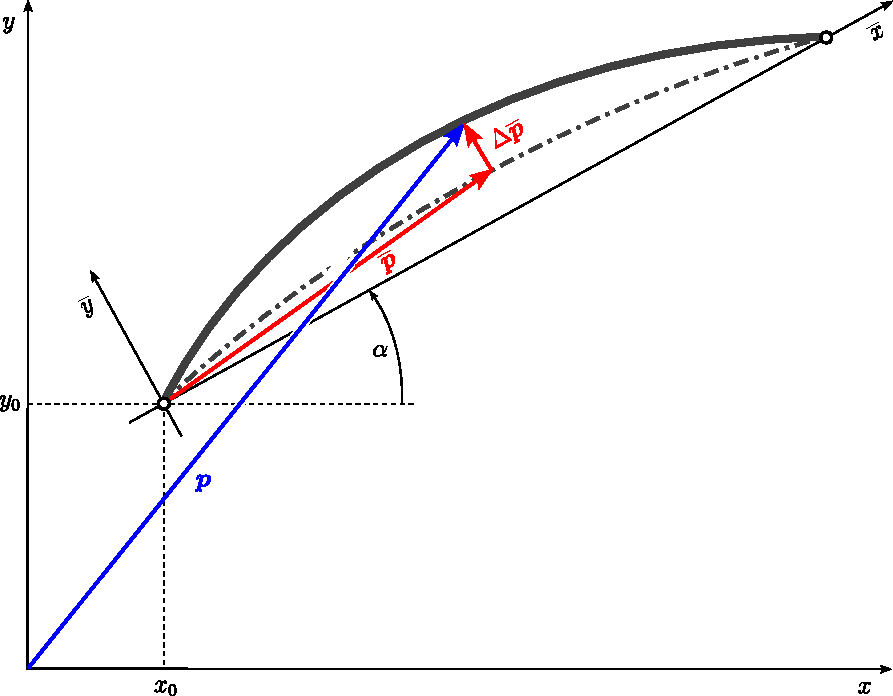
\includegraphics[width=0.8\textwidth]{figures/elements/beam-element-displacement-transform}
\caption{Position of the beam axis in local and global coordinates}
\label{fig:beam-element-displacement-transform}
\end{figure}

The position and orientation $\boldsymbol{p}$ in global coordinates is then obtained by accounting for the rotation~$\alpha$ and the translation~$(x_0,\,y_0)$ of the local reference frame:

\begin{align}
\boldsymbol{p}(s,\,t) &=
\underbrace{
\begin{bmatrix}
\cos(\alpha(t)) & -\sin(\alpha(t)) & 0 \\
\sin(\alpha(t)) & \cos(\alpha(t)) & 0 \\
0 & 0 & 1
\end{bmatrix}
}_{\boldsymbol{R}(\alpha(t))}
\bigg(\overline{p}(s) + \Delta\overline{p}(s)\bigg)
+
\underbrace{
\begin{bmatrix}
x_0(t) \\
y_0(t) \\
\alpha(t)
\end{bmatrix}
}_{\boldsymbol{b}(t)} \notag \\
&= \boldsymbol{R}\big(\overline{\boldsymbol{p}} + \boldsymbol{E}_u\,\overline{\boldsymbol{u}}\big) +  \boldsymbol{b}
\end{align}

By differentiation, the global velocity~$\dot{\boldsymbol{p}}$ follows as

\begin{align}
\dot{\boldsymbol{p}}(s,\,t) &= \dot{\boldsymbol{R}}\Big(\overline{\boldsymbol{p}} + \Delta\overline{\boldsymbol{p}}\Big) + \boldsymbol{R}\Delta\dot{\overline{\boldsymbol{p}}} + \dot{\boldsymbol{b}}(t) \notag \\
&= \dot{\alpha}\boldsymbol{R}'\Big(\overline{\boldsymbol{p}} + \Delta\overline{\boldsymbol{p}}\Big) + \boldsymbol{R}\Delta\dot{\overline{\boldsymbol{p}}} + \dot{\boldsymbol{b}},
\end{align}

with the following auxiliary terms:

\begin{align}
\boldsymbol{R}' &= \begin{bmatrix}
-\sin(\alpha) & -\cos(\alpha) & 0 \\
\cos(\alpha) & -\sin(\alpha) & 0 \\
0 & 0 & 0
\end{bmatrix}
&
\dot{\alpha} &= \frac{\partial\alpha}{\partial\boldsymbol{u}}^\intercal\,\dot{\boldsymbol{u}} \\
\dot{\overline{\boldsymbol{p}}} &= \boldsymbol{E}_{u}\boldsymbol{J}\dot{\boldsymbol{u}}
&
\frac{\partial\alpha}{\partial\boldsymbol{u}} &=
\frac{1}{\Delta x^2 + \Delta y^2}
\begin{bmatrix}
\phantom{-}\Delta y \\
-\Delta x \\
0 \\
-\Delta y \\
\phantom{-}\Delta x \\
0
\end{bmatrix}
\end{align}

These transformations enable the evaluation of the beam's bending line inbetween the nodes, leading to finer-grained simulation output irrespective of the number of elements being used.

\newpage
\subsection{Cross-Section Properties}

When we derived the elastic properties of the beam segment, we did it in a fairly general way.
The only assumption about the beam's cross-sections was, that they exhibit a linear relationship between forces and strains, as formlized by equation~\eqref{eq:section-stiffness-matrix}, where this relationship is described by the stiffness matrix $\boldsymbol{C} \in \mathbb{R}^{3 \times 3}$ of the section.
But in practice we have to calculate these matrices for a subset of cross-sections that is relevant to VirtualBow, which we are going to do here.
The following derivations have been adapted from~\cite{bib:tm2} and~\cite{bib:wiki-sandwich}.

Consider a laminated cross section as shown in figure~\ref{fig:composite-sections-1}.
It is symmetric with respect to the~$y$-axis, bends/rotates around the~$z$-axis and consists of a number of rectangular layers.
Each layer has its own density~$\rho_i$ and elastic modulus~$E_i$.
The geometry of the layers is given by their width~$w_i$, height~$h_i$ and center position~$y_i$.

\begin{figure}[h]
\centering
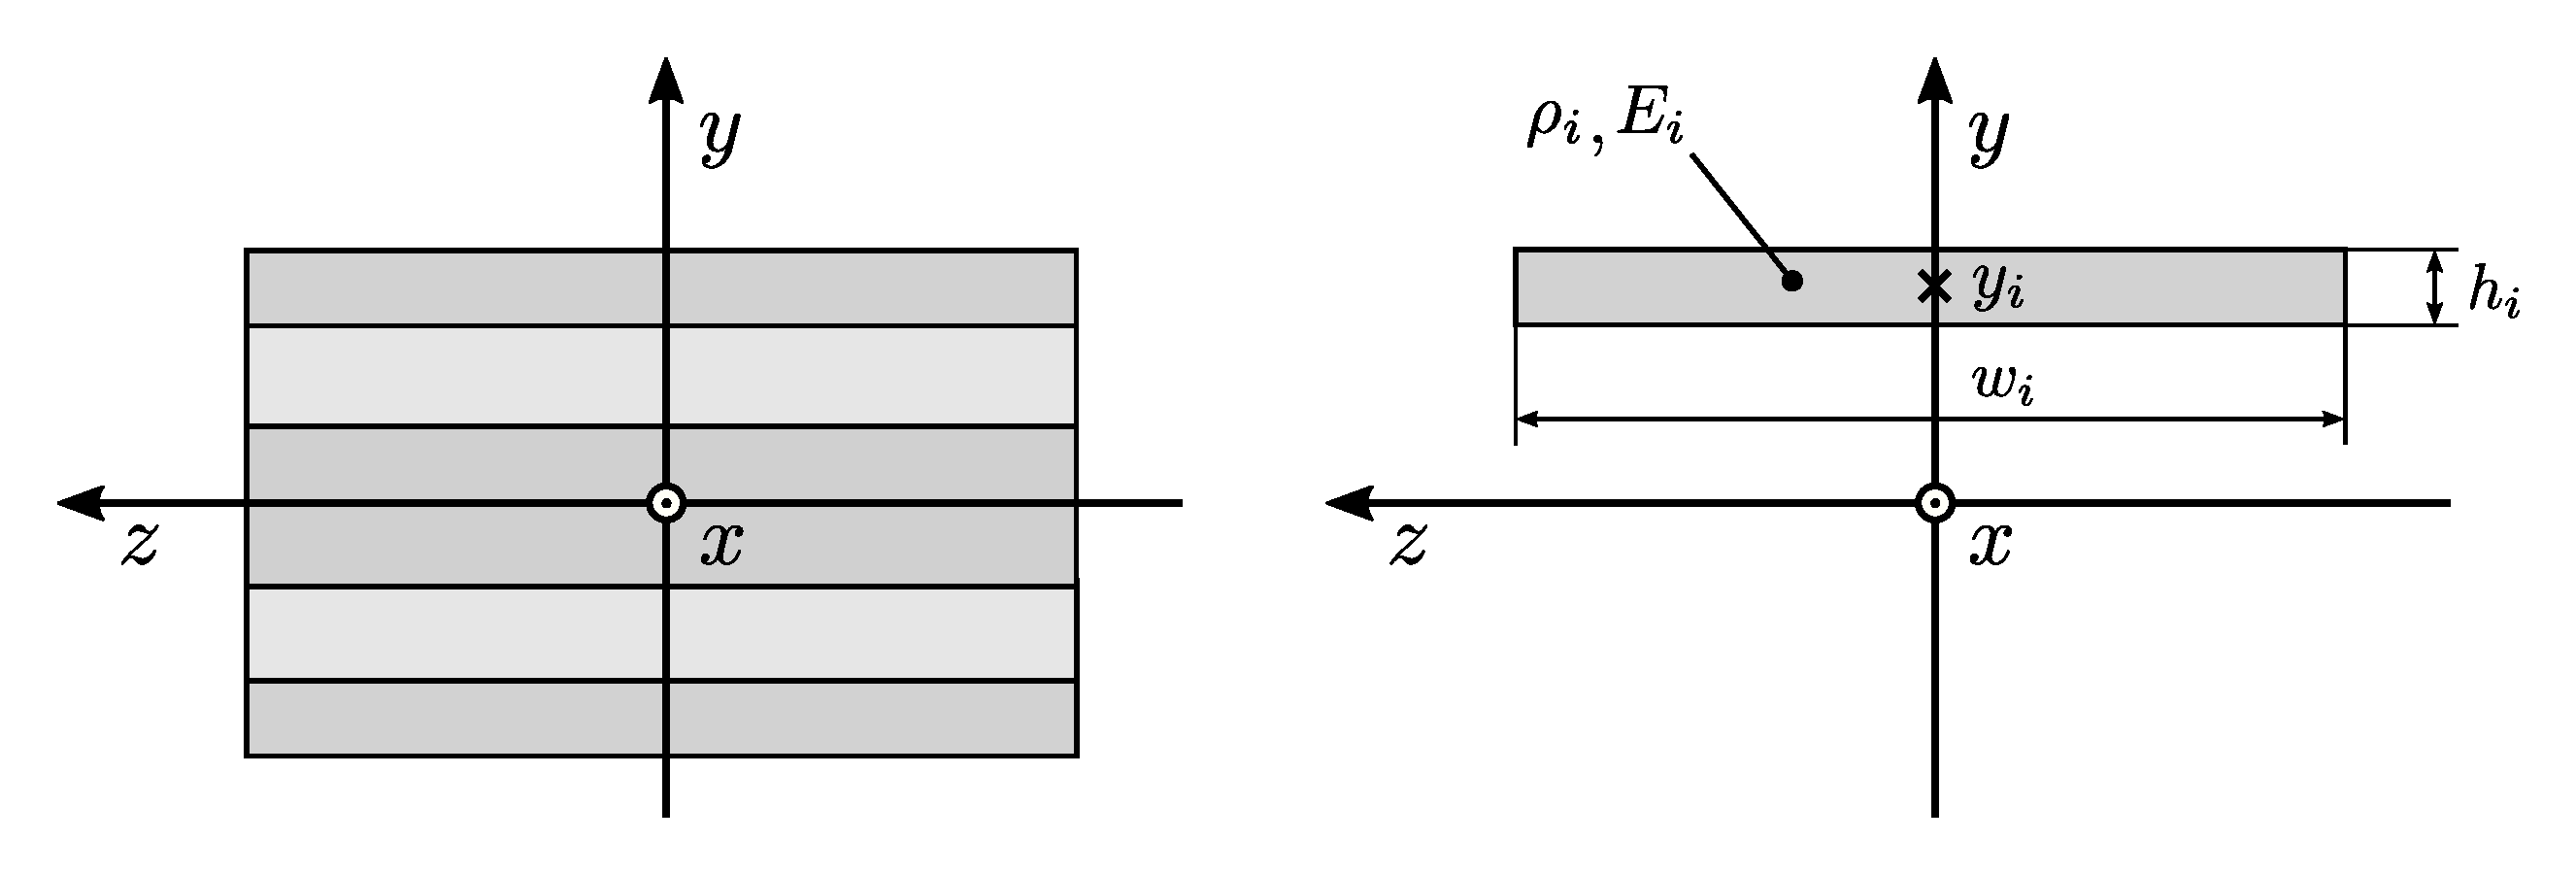
\includegraphics[width=0.9\textwidth]{figures/elements/composite-sections-1}
\caption{Composite cross section and single layer}
\label{fig:composite-sections-1}
\end{figure}

In Euler-Bernoulli beam theory the cross sections are assumed to stay flat and perpendicular to the beam axis during deformation.
We assume this to be true for our laminated cross section as well.
The distribution of longitudinal strain over the section is therefore given by the continuous function

\begin{equation}
\overline{\varepsilon}(y) = \varepsilon - \kappa\,y,
\end{equation}

where~$\varepsilon$ is the strain of the beam's centerline in $x$-direction and $\kappa$ its curvature around the $z$-axis.
The stress distribution however is not necessarily continuous, because each layer can have a different elastic modulus.
According to Hooke's law, the stress within a layer is given by

\begin{equation}
\sigma_i(y) = E_i\cdot\overline{\varepsilon}(y),\quad y \in [y_i - \frac{h_i}{2},\,y_i + \frac{h_i}{2}].\label{eq:beam-stress-distribution}
\end{equation}

In order to determine the elastic constants $C_{ij}$ from the section's stiffness matrix, we calculate the normal force~$N$ and bending moment~$M$ acting on the cross section by integrating the stresses~(\ref{eq:beam-stress-distribution}) over the section's area.
For the normal force this amounts to

\begin{align}
N &= \int_A \sigma\,\mathrm{d}A = \sum_i\int_{A_i}\sigma_i\,\mathrm{d}A_i = \sum_i\int_{A_i}E_i\,\overline{\varepsilon}(y)\,\mathrm{d}A_i = \sum_i E_i \int_{A_i}(\varepsilon - \kappa\,y)\,\mathrm{d}A_i,\notag\\
&= \left(\sum_i E_i\int_{A_i}\mathrm{d}A_i\right)\varepsilon - \left(\sum_i E_i\int_{A_i}y\,\mathrm{d}A_i\right)\kappa,\notag\\
&=
\underbrace{
\left(\sum_i E_i\,A_i\right)
}_{C_{\varepsilon\varepsilon}}
\varepsilon
\underbrace{
- \left(\sum_i E_i\,A_i\,y_i\right)
}_{C_{\varepsilon\kappa}}
\kappa.\label{eq:elements:beam:constitutive_1}
\end{align}

This gives us the term~$C_{\varepsilon\varepsilon}$ for the stiffness of the section against tension and the coupling term~$C_{\varepsilon\kappa}$ between tension and bending.
The same can be done for the bending moment,

\begin{align}
M &= -\int_A y\,\sigma\,\mathrm{d}A = -\sum_i\int_{A_i}y\,\sigma_i\,\mathrm{d}A_i,\notag\\
&= -\sum_i\int_{A_i}y\,E_i\,(\varepsilon - \kappa\,y)\,\mathrm{d}A = -\sum_i\int_{A_i}(E_i\,\varepsilon\,y - E_i\,\kappa\,y^2)\,\mathrm{d}A,\notag\\
&= -\left(\sum_i E_i\int_{A_i}y\,dA_{i}\right)\varepsilon + \left(\sum_i E_i\int_{A_i}y^2\,dA_i\right)\kappa,\notag\\
&=
\underbrace{
-\left(\sum_i E_i\,A_i\,y_i\right)
}_{C_{\varepsilon\kappa}}
\varepsilon +
\underbrace{
\left(\sum_i E_i\,I_{i}\right)
}_{C_{\kappa\kappa}}
\kappa.\label{eq:elements:beam:constitutive_2}
\end{align}

This gives us the same coupling term~$C_{\varepsilon\kappa}$ as well as the stiffness~$C_{\kappa\kappa}$ against bending.
One section force is still missing: the shear force $Q$.
Unfortunately, the distribution of shear stresses over a cross-section like this is pretty complicated.
But as already mentioned, VirtualBow doesn't make use of the shear component right now, so it is more like a placeholder.
So we are going to make a crude approximation for the shear stiffness, based on a constant shear stress within each layer:

\begin{align}
Q &= \int_A \tau\,\mathrm{d}A = \sum_i\int_{A_i}\tau_i\,\mathrm{d}A_i = \sum_i\int_{A_i}G_i\,\gamma\,\mathrm{d}A_i = \underbrace{
\left(\sum_i G_i\,A_i\right)\gamma
}_{C_{\gamma\gamma}}.\label{eq:elements:beam:constitutive_3}
\end{align}

The idea is to make this approximation obsolete in the future by switching to a numerical cross-section analysis instead, which accurately computes all stiffnesses and stress distributions of the section, including those for shear and torsion, and doesn't make any kinematic assumptions as in the Euler-Bernoulli or Timoshenko theories.
But for now we end up with the following analytical stiffnesses:

\begin{align}
C_{\varepsilon\varepsilon} &= \sum_i E_i\,A_i, & C_{\kappa\kappa} &= \sum_i E_i\,I_{i} \\
C_{\gamma\gamma} &= \sum_i G_i\,A_i & C_{\varepsilon\kappa} &= -\sum_i E_i\,A_i\,y_i
\end{align}

And therefore the section stiffness matrix

\begin{equation}
\boldsymbol{C} =
\begin{bmatrix}
C_{\varepsilon\varepsilon} & C_{\varepsilon\gamma} & 0 \\
C_{\varepsilon\gamma} & C_{\gamma\gamma} & 0 \\
0 & 0 & C_{\kappa\kappa} \\
\end{bmatrix}.
\label{eq:section-stiffness-matrix-analytic}
\end{equation}

as defined in~\eqref{eq:section-stiffness-matrix}.
In the case of the rectangular layers shown above, area~$A_i$ and second moment of inertia~$I_i$ evaluate to

\begin{align}
A_i &= w_i\,h_i, \quad I_i = A_i\left(\frac{h_i^2}{12} + y_i^2\right).
\end{align}

For completing the element's mass matrix, we're also going to need the linear density (mass per unit length) of the laminated section.
It can be calculated by summing the the densities of the individual layers as

\begin{equation}
\mu = \sum_i \rho_i A_i.\label{eq:beam-linear-density}
\end{equation}

Pretty straightforward, compared to the other terms.

\newpage
\subsection{Lumped Masses}

When trying to come up with the diagonal entries of our lumped mass matrix~\eqref{eq:corotational-mass-matrix}, we are basically asking how to pick concentrated masses and inertias~$m_0$,~$J_0$ and~$m_1$,~$J_1$ at the nodes of the element such that it behaves like the actual beam segment, whose mass is continuously distributed along the curved and moving beam axis.
It is not surprising that this isn't possible in an exact sense.
There is a reason, after all, why the consistent mass matrix for a corotational beam element is as complex as it is.
So we will have to make reasonable approximations.

First of all, we can compute the total mass of the beam segment by integrating the section's linear density~\eqref{eq:beam-linear-density} over its length, which yields

\begin{equation}
m = \int_{0}^{l} \mu(s)\,ds.
\end{equation}

An obvious way for lumping this mass is to assign the first half of the integral to the first node and the second half to the second node, giving us the nodal masses

\begin{equation}
m_0 = \int_{0}^{\frac{l}{2}} \mu(s)\,ds, \quad m_1 = \int_{\frac{l}{2}}^{l} \mu(s)\,ds.
\end{equation}

The rotary inertia is a little more tricky, since there is no obvious "total inertia" that can just be distributed between nodes.
In~\cite{bib:colorado31}, a common choice for straight, uniform Euler-Bernoulli beams is presented as

\begin{equation}
I_{0} = I_{1} = c \cdot \rho A l^3
\end{equation}

with a fudge factor~$c$ (symbol adapted), typically chosen between~$0$ and~$\nicefrac{1}{50}$, but impossible to determine in such a way that all physical constraints are fulfilled equally.
The expression~$\rho A l^3$ is proportional to the beam's rigid rotary inertia, but the exact point of reference is baked into~$c$.
We attempt to generalize this by defining our nodal moments of inertia as
%
\begin{align}
J_0 &= c \cdot \int_{0}^{l} \mu(s) \lVert \boldsymbol{r}(s) - \boldsymbol{r}(0) \rVert^2\,ds, \\
J_1 &= c \cdot \int_{0}^{l} \mu(s) \lVert \boldsymbol{r}(s) - \boldsymbol{r}(l) \rVert^2\,ds,
\end{align}

where $c$ is a different fudge factor and the integrals are the rigid-body inertia of the segment with respect to each of the nodes, respectively.

\newpage
\subsection{Damping Matrix}

The only thing still missing from the beam element is the damping matrix~$\overline{\boldsymbol{D}}$ of the beam segment, analogous to its stiffness matrix, as required for the calculatio of the local forces~\eqref{eq:corotational-linear-forces}.
Since the stiffness matrix has been derived from the segment's material properties and geometry, it would seem logical to do the same for the damping matrix.
But characterizing the dissipative properties of materials is much more tricky than their elastic properties.
Most common materials do not follow a simple, linear damping law that would lead to a linear damping matrix in the first place.
So it can only ever be a crude approximation, so that at least some energy dissipation is included in the bow model.

So instead of deriving the damping matrices from actual material properties, we are going to identify them based on the damping properties of the overall system, i.e. the bow limb.
The damping model that is utilized for this is called \textit{Rayleigh damping} or \textit{proportional damping}, which is a simple approach that is very popular when only little is known about the underlying physical details of the damping.
The idea is to write the damping matrix of a linear(ized) system as a weighted sum of its stiffness- and mass matrix,

\begin{equation}
\boldsymbol{D} = \alpha\boldsymbol{K} + \beta\boldsymbol{M}\label{eq:rayleigh-damping-matrix}
\end{equation}

with the factor $\alpha$ for stiffness-proportional damping and the factor $\beta$ for mass-proportional damping.
The stiffness-proportional part dampens the system as if the material behaved in a viscous way while the mass-proportional part dampens the system as if the system were moving through a viscous medium.
It can be shown \cite{bib:rayleigh-damping} that natural frequencies and corresponding damping ratios in such a system are related by 

\begin{equation}
\zeta_{i} = \frac{1}{2}\left(\alpha\,\omega_{i} + \frac{\beta}{\omega_{i}}\right).
\end{equation}

This relationship can be used for identifying $\alpha$ and $\beta$ from prescribed values of the damping ratio at specific modes.
In our case we use stiffness-proportional damping only, so $\beta$ is set to zero.
If we pick a damping ratio of $\zeta_{0}$ for the first mode of the system, we can determine the required Rayleigh parameter $\alpha$ as

\begin{equation}
\zeta_{0} = \frac{1}{2}\alpha\,\omega_{0} \quad \Rightarrow \quad \alpha = \frac{2\zeta_{0}}{\omega_{0}}. \label{eq:rayleigh-alpha-identification}
\end{equation}

In practice this works as follows for the bow limb.
The value~$\zeta_{0}$ is set by users as the damping ratio of the first eigenmode of the limb.
This is supposed to be an empirical value that can be experimentally determined on real bows and then chosen from experience for simulations.
When the bow simulation is set up, the limb is initialized without damping at first.
With this undamped limb model, before the string is attached, a modal analysis is performed to determine its first undamped natural frequency~$\omega_{0}$.
Using this frequency and the prescribed damping ratio~$\zeta_{0}$, the required damping coefficient~$\alpha$ is determined from equation (\ref{eq:rayleigh-alpha-identification}).
The damping matrices of each beam element are then initialized as~$\overline{\boldsymbol{D}} = \alpha\overline{\boldsymbol{K}}$.
When the system is linearized, as is the case here, the factor~$\alpha$ carries over to the system level as in~\eqref{eq:rayleigh-damping-matrix}.

\newpage
\section{String Element}

\subsection{Internal Forces}

An idealized string only transfers tensile forces and has no resistance to shear and bending.
Figure~\ref{string-element-constitutive} shows such a string with an initial length of~$l_0$.
When subjected to a normal force~$N$ it elongates by~$\Delta l$.

\begin{figure}[h]
\centering
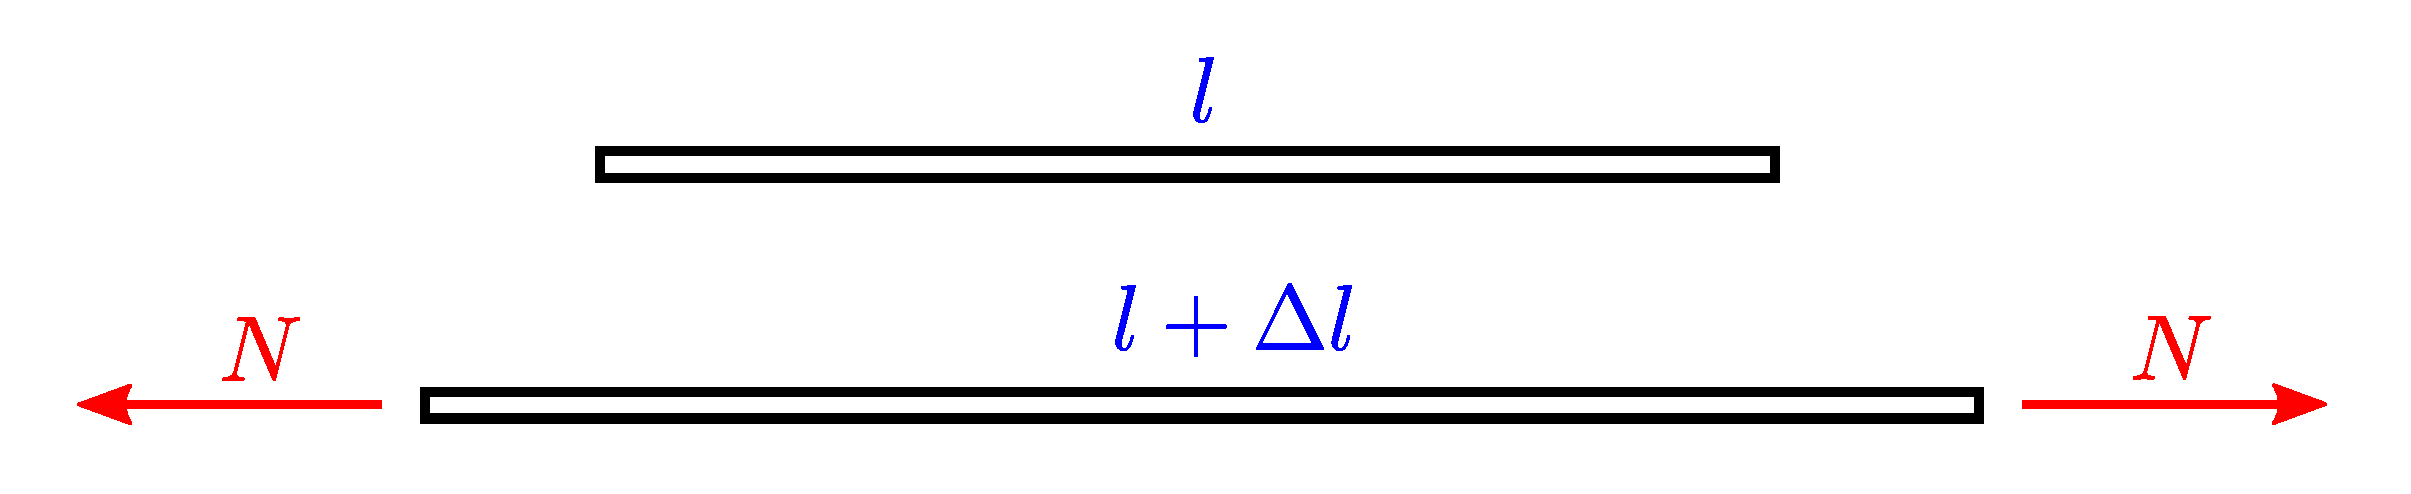
\includegraphics[width=0.75\textwidth]{figures/elements/string-element-constitutive}
\caption{Elongation of a bar under load}
\label{string-element-constitutive}
\end{figure}

We assume the strain~$\varepsilon = \frac{\Delta l}{l}$ to be constant over the length of the string.
In order to simulate the elastic as well as the damping properties of the string, a viscoelastic material model of the form

\begin{equation}
\sigma = E\,\varepsilon + \eta\,\dot{\varepsilon}
\end{equation}

is chosen.
Here~$E$ is the elastic modulus and~$\eta$ the viscosity of the material.
This model is called the \textit{Kelvin-Voigt model} and combines linear elastic and linear viscous behaviour.
We will later identify~$\eta$ based on the prescribed damping ratio of the string, similar to how we identified the damping properties of the beam elements.
The normal force in the string, given a constant cross section area~$A$, is therefore

\begin{align}
N = \sigma A &= EA\,\varepsilon + \eta A\,\dot{\varepsilon}.\label{eq:bar-constitutive}
\end{align}

The product~$EA$ is also called the longitudinal stiffness.
To use this as the string model in our bow simulation, we have to pick a set of nodes and formulate the internal forces in terms of the nodal displacements.
It seems reasonable to place the string between two nodes, one start- and one endpoint, but there is an additional complication: the string model must also handle recurve bows, so we have to consider its possible contact with the bow limb.
This means that the current shape of the string, as well as its internal forces, don't only depend on its own start- and endpoint, but also on the nodes of the limb.
Figure~\ref{fig:elements:string-element} shows the resulting setup for our element.
The first node, with the position~$(x_0,\,y_0)$, is the starting point of the string.
This is the same node where the arrow is attached in the final model.
This is followed by the nodes~$(x_i,\,y_i,\,\varphi_i),\,i = 1 \ldots n-1$ of the limb's reference line.
Since the string doesn't contact the limb at its reference line, but at its outer surface, each of those also carries a distance~$d_i$, which defines a possible contact point perpendicular to the reference line.
The contact point of the last limb node~$(x_{n-1},\,y_{n-1},\,\varphi_{n-1})$ is the endpoint of the string, this would be the limb tip in the bow model.

\begin{figure}[h]
\centering
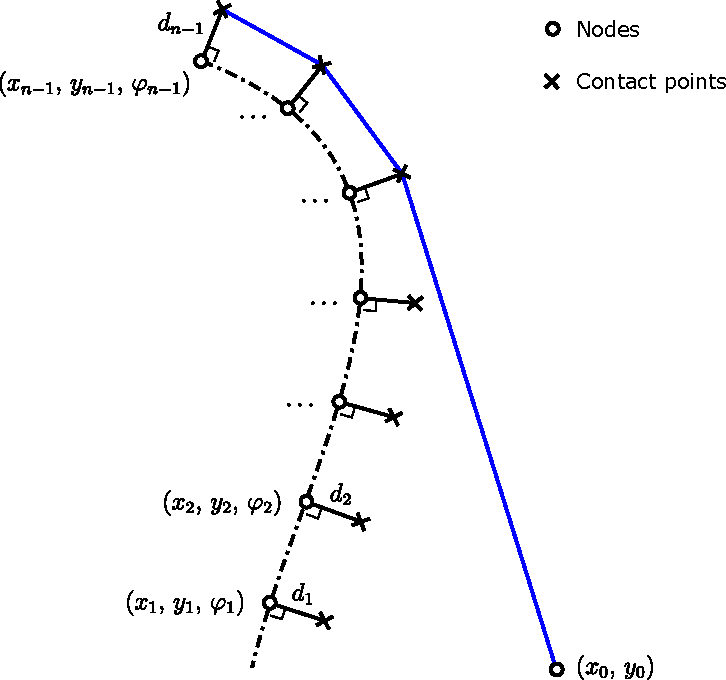
\includegraphics[width=0.8\linewidth]{figures/elements/string-element}
\caption{Contact interface between limb and string}
\label{fig:elements:string-element}
\end{figure}

One shortcoming of this approach is already apparent: the contact with the string is only determined by the positions of the limb nodes, not by the actual deformed geometry of the limb's beam elements.
This could be a possible future improvement that would allow us to accurately resolve the string contact with a much smaller number of limb nodes/elements.

We define the displacement vector~$\boldsymbol{u}$ of the element, describing the string's current configuration, as

\begin{equation}
\boldsymbol{u} = \begin{bmatrix}
x_{0}, & y_{0}, & x_{1}, & y_{1}, & \varphi_{1}, & \cdots & x_{n-1}, & y_{n-1}, & \varphi_{n-1}
\end{bmatrix}^\intercal
\end{equation}

The first step in evaluating the internal forces of this element is to determine which of the limb nodes make contact with the string.
First of all, the limb nodes are not the points where the string makes physical contact.
The actual contact points at the belly surface of the limb are given by

\begin{align}
\bar{x}_{0} &= x_{0}, \quad \bar{x}_{i} = x_{i} - d_{i}\sin(\varphi_{i}) \\
\bar{y}_{0} &= y_{0}, \quad \bar{y}_{i} = y_{i} + d_{i}\cos(\varphi_{i})
\end{align}

with the perpendicular distances $d_{i}$ as obtained from the limb's cross section geometry.
The task of finding the contact points is then equivalent to finding the convex envelope of the points $\{x_{0},\,y_{0},\,\bar{x}_{1},\,\bar{y}_{1},\,\ldots,\,\bar{x}_{n-1},\,\bar{y}_{n-1}\}$.
This is currently implemented by a method similar to the \textit{Graham scan}~\cite{bib:grahamscan}, but adapted for 1D lines.
This scan is currently done on each evaluation of the element.
A possible improvement over this would be an algorithm that keeps track of the contact points and only considers what has changed since the last evaulation.  
Having found the contact points, we now know the exact geometrical configuration of the string and can begin formulating the internal forces for the element.
Let's denote all points that are part of the convex envelope with the index $k$.
The length between two surface points $i$ and $j$ is given by

\begin{equation}
l_{ij} = \sqrt{(\bar{x}_j - \bar{x}_i)^2 + (\bar{y}_j - \bar{y}_i)^2}
\end{equation}

The total length of the string is the sum of all line segments of the convex envelope,

\begin{equation}
l(\boldsymbol{u}) = \sum_{k} l_{k-1,k}.
\end{equation}

The strain and strain rate are expressed in terms of the overall length~$l$ as

\begin{equation}
\varepsilon = \frac{l(\boldsymbol{u}) - l_{0}}{l_{0}}, \quad \dot{\varepsilon} = \frac{1}{l_{0}}\frac{\partial l}{\partial \boldsymbol{u}}\dot{\boldsymbol{u}}
\end{equation}

The virtual work of the internal forces is obtained by integrating the product of stress $\sigma$ and the strain variation $\delta \varepsilon$ over the element's volumne, leading to

\begin{align}
\delta W_{I} &= \int_{V} \sigma\,\delta\varepsilon\,dV = \int_{0}^{l_{0}}\int_{A} \sigma\,\delta\varepsilon\,dA\,ds = \left(EA\,\varepsilon + \eta A\,\dot{\varepsilon}\right)l_{0}\frac{\partial\varepsilon}{\partial\boldsymbol{u}}\delta\boldsymbol{u}.
\end{align}

The internal forces themselves are therefore

\begin{equation}
\boldsymbol{Q}(\boldsymbol{u},\,\dot{\boldsymbol{u}}) = \left(EA\varepsilon + \eta A\dot{\varepsilon}\right)l_{0}\frac{\partial\varepsilon}{\partial\boldsymbol{u}} = \underbrace{\left(k(l - l_{0}) + d\dot{l}\right)}_{N(\boldsymbol{u},\,\dot{\boldsymbol{u}})}\frac{\partial l}{\partial\boldsymbol{u}}
\end{equation}

where~$k = \frac{EA}{l_{0}}$ and~$d = \frac{\eta A}{l_{0}}$ are the stiffness and damping, respectively, corresponding to a linear spring-damper, and $N$ is the normal force within the string.
The tangent stiffness matrix is derived from the internal forces as

\begin{align}
\boldsymbol{K} = \frac{\partial\boldsymbol{Q}}{\partial\boldsymbol{u}} &= \left(k\frac{\partial l}{\partial\boldsymbol{u}}^\intercal + d\frac{\partial\dot{l}}{\partial\boldsymbol{u}}^\intercal\right)\frac{\partial l}{\partial\boldsymbol{u}} + \left(k(l - l_{0}) + d\dot{l}\right)\frac{\partial^2 l}{\partial\boldsymbol{u}^2}, \notag \\
&= \left(k\frac{\partial l}{\partial\boldsymbol{u}}^\intercal + d\dot{\boldsymbol{u}}^\intercal\frac{\partial^2 l}{\partial\boldsymbol{u}^2}\right)\frac{\partial l}{\partial\boldsymbol{u}} + \left(k(l - l_{0}) + d\dot{l}\right)\frac{\partial^2 l}{\partial\boldsymbol{u}^2}.
\end{align}

Similarly, the tangent damping matrix is obtained as

\begin{equation}
\boldsymbol{D} = \frac{\partial\boldsymbol{Q}}{\partial\dot{\boldsymbol{u}}} = d\frac{\partial\dot{l}}{\partial\dot{\boldsymbol{u}}}^\intercal\frac{\partial l}{\partial\boldsymbol{u}} = d\,\frac{\partial l}{\partial\boldsymbol{u}}^\intercal\frac{\partial l}{\partial\boldsymbol{u}}.
\end{equation}

The derivatives~$\nicefrac{\partial l}{\partial\boldsymbol{u}}$ and~$\nicefrac{\partial^2 l}{\partial\boldsymbol{u}^2}$ of the string length, which are required for evaluating these expressions, are carried out in detail in Appendix~\ref{sec:derivatives-for-the-string-element}.

One final tweak to the string model is required for dynamic analysis.
Right now the model resists tension as well as compression, even though one of the defining properties of a string or cable is that it only resists tension, but not compression.
For static analysis this is not an actual problem, since the string should be under tension in any equilibrium state of the bow anyway.
In dynamic analysis however, especially in the slightly chaotic phase after the arrow leaves the string, it can happen that the string length becomes shorter than it's initial length, which means that it is under compression.
This must not generate forces that counteract that compression, otherwise the string would behave like a bar and not linke a string.
In other words, the stiffness of the string on compression should be zero.
Since a stiffness of exactly zero however leads to a singular tangent stiffness matrix for the system, which creates problems, we set it to a very small value instead by multiplying it with a small factor~$c << 1$.
Doing the same for the damping, the longitudinal stiffness $EA^*$ and damping $\eta A^*$ used for dynamic analysis become

\begin{equation}
EA^* = \begin{cases}
    \phantom{c\cdot}EA, & \text{if $\Delta l \ge 0$} \\
    c\cdot EA, & \text{otherwise}
\end{cases}, \quad
\eta A^* = \begin{cases}
    \phantom{c\cdot}\eta A, & \text{if $\Delta l \ge 0$} \\
    c\cdot \eta A, & \text{otherwise}
\end{cases}
\end{equation}

depending on the sign of the elongation~$\Delta l$.
This introduces a non-smooth transition at~$\Delta l = 0$, which is not ideal, but hasn't caused any obvious problems in practice either.

\newpage
\subsection{Lumped Masses}

We make no attempt at deriving a consistent mass matrix for this element, or any mass matrix at all.
There is no way it would have any nice properties, like being constant or diagonal.
Instead we keep the element massless and move the responsibility of accounting for the string's mass to the bow model, where this is done by dividing it between two point masses placed at the center and the end of the string.

\begin{figure}[h]
\centering
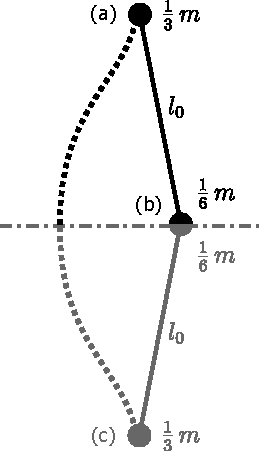
\includegraphics[width=0.3\linewidth]{figures/elements/string-element-masses}
\caption{Lumping of the string's total mass to three points}
\label{fig:elements:string-element-masses}
\end{figure}

When determining those point masses, we have to keep in mind that the string element we derived only models and simulates one half of the string, while the actual bow is mirrored as shown in figure~\ref{fig:elements:string-element-masses}.
Since the length~$l_0$ of the element is only half the total length of the string, the total string mass is $m = 2\,\rho A l_{0}$.
According to figure~\ref{fig:elements:string-element-masses} there are three obvious points for distributing this mass: the upper end (a) of the string, the string center (b) and the lower end (c).
If the total mass is evenly divided, each of those points is given a mass of~$\nicefrac{1}{3}\,m$.
But only the mass (a) and half of (b) are actually part of the upper half of the bow that is being simulated.
So the actual masses for the model are~$\nicefrac{1}{3}\,m$ for the upper string end (a) and~$\nicefrac{1}{6}\,m$ as the upper half of the center mass (b).
The same distribution of the string's mass was also used by Kooi \cite{bib:kooi81}, which seems to confirm this reasoning.

\newpage
\subsection{Damping}

The question of identifying the viscosity $\eta$ of the string material is still open.
The idea is, similar to the limb, to prescribe a certain damping ratio for the string and identify the viscosity based on that.
But unlike the limbs, we don't need a numerical modal analysis of the string to do this, since we can carry it out analytically.
As shown in Appendix~\ref{chapter:viscoelastic-bar-vibrations}, the damping ratio of the first longitudinal eigenmode of a continuous string of initial length $l_0$ is

\begin{equation}
\zeta = \frac{\pi}{4l_0}\,\frac{\eta A}{\sqrt{\rho A \cdot EA}}
\end{equation}

which, when solved for $\eta A$ gives us the effective viscosity of the string as

\begin{equation}
\eta A = \frac{4l_0}{\pi}\sqrt{\rho A \cdot EA}\cdot\zeta,
\end{equation}

where~$\zeta$ is the desired damping ratio.
It is worth noting that these longitudinal eigenmodes only apply to a continuum model of a string and are not actually present in the string element as we modeled it.
But that doesn't matter for our purpose here.